\documentclass{dcthesis}

%This version of the thesis template has been updated for the February 2017 thesis guidelines provided by the School of Graduate and Advanced Studies by David Freund and Daryl DeFord.

%  Some good options are draft and singlespacing, for drafts, and *final*,
%for the final cut, and noheadings, for a printout without headings.
%You can also use the copyright option to add a copyright.  Note:
%final will enforce a bunch of different options, like oneside, 12pt
%and doublespacing, as well as make the margins correct.   Draft, has
%larger margins and is appropriate for twosided printing.


%%%%%%%%%%%%%%%%%%%%%%%%%%%
%%%%    IMPORTANT     %%%%%
%%%%%%%%%%%%%%%%%%%%%%%%%%%
%
%  Because dvips doesn't know/care about the page size of the dvi file
%  its working on, and because its so important that the margins of
%  your thesis are correct you have to make sure that you are using
%  the command dvi -t letter *thesisnamehere*
%
%  If you are using a terminal this is straightforward, but if you are
%  using a tex editing program it make take a little bit of searching
%  before you figure out how to make this work.
%
%  Alternatively, you might consider compiling using pdflatex, which
%  compiles straight to a PDF and doesn't have this problem.
\committee[F. Jon Kull, Ph.D.]{}{}{}{}
\school{Dartmouth College}{Hanover, New Hampshire}
\degree{Doctor of Philosophy}
\field{Mathematics}
\usepackage{graphicx}   % Needed for figures.
\usepackage{index}
\usepackage{amsmath}    % Needed for align.
\usepackage{amssymb}    % Needed for mathbb.
\usepackage{amsthm}     % For the theorem environment.
\usepackage[nottoc]{tocbibind} % Bibliography in toc.
\usepackage{listings}   % Display code in a LaTeX document.
\usepackage{xcolor}     % RGB defined colors.
\usepackage{hyperref}   % Hyperlinks for URLs and references.

% Setup parameters for hyperlinks.
\hypersetup{colorlinks = true, linkcolor = blue}
\theoremstyle{plain}
\newtheorem{theorem}{Theorem}[section]
\newtheoremstyle{normal}{\topsep}{\topsep}{}{}{\bfseries}{}{0.5em}{}
\theoremstyle{normal}
\newtheorem{definitionx}{Definition}[section]
\newtheorem{conjecture}{Conjecture}[section]
\newtheorem{question}{Question}[section]

\newenvironment{definition}{%
    \pushQED{\qed}\renewcommand{\qedsymbol}{$\blacksquare$}\definitionx%
}{%
    \popQED\enddefinitionx%
}

\definecolor{background}{rgb}{0.9, 0.9, 0.9}
\lstdefinestyle{CStyle}{
    backgroundcolor=\color{background},
    commentstyle=\color{gray},
    keywordstyle=\color{blue},
    numberstyle=\tiny\color{red},
    stringstyle=\color{orange},
    basicstyle=\footnotesize,
    breakatwhitespace=false,
    breaklines=true,
    captionpos=b,
    keepspaces=true,
    numbers=left,
    numbersep=5pt,
    showspaces=false,
    showstringspaces=false,
    showtabs=false,
    tabsize=2,
    language=C
}

\title{Khovanov Homology and Legendrian Simple Knots}
\author{Ryan Maguire}
\date{\today}
\setlength{\parindent}{0em}
\setlength{\parskip}{0em}
\graphicspath{{../../images/}}
\renewcommand{\labelenumi}{(\alph{enumi})}
\renewcommand{\labelenumii}{(\roman{enumii})}
\renewcommand{\chaptermark}[1]{\markboth{{\sc #1}}{{\sc #1}}}
\renewcommand{\sectionmark}[1]{\markright{{\sc \thesection\ #1}}}
\makeindex
\title{Khovanov Homology and Legendrian Simple Knots}
\author{Ryan Maguire}
\date{\today}
\field{Mathematics}
\degree{Doctor of Philosophy}
\committee{Vladimir Chernov}{Peter Doyle}{Ina Petkova}{Patricia Cahn}

\begin{document}
    \frontmatter
    \maketitle
    \chapter*{Abstract}
        The Jones polynomial and Khovanov homology are powerful invariants
        in knot theory. Their computations are known to be NP-Hard and it
        can be quite a challenge to directly compute either of them for a
        general knot. We develop explicit algorithms for the Jones polynomial
        and discuss the implementation of algorithm for Khovanov homology.
        Using this we tabulate the invariants for millions of knots, generate
        statistics on them, and formulate conjectures for Legendrian and
        transverally simple knots.
    \addcontentsline{toc}{section}{Abstract}
    \chapter*{Preface}
        \addcontentsline{toc}{section}{Preface}
        This work examines some of the computational aspects of knot theory and
provides evidence for new conjectures in the field. Chapter 1 contains a quick
summary of the results and introduces the problems that are to be studied.
In chapter 2 we discuss some elementary background, including several of the
combinatorial methods of representing knots that allow one to make use of
computers in their calculations. The challenge of discerning knots is then
tackled in chapter 3 where we discuss knot invariants. Here we introduce two
new algorithms for the computation of the Jones polynomial,
including a new modification of the Tait graph for virtual knots.
These new algorithms are still exponential in time (with respect to the number
of crossings in a knot diagram), but linear in their spatial requirement.
We also explore some known ideas for the calculation
of other invariants such as the Alexander and HOMFLY-PT polynomials, as well as
Khovanov homology, by reviewing definitions and analyzing algorithms.
In chapter 3 we discuss contact topology and Legendrian
simple knots, and then get in to the heart of
the thesis in chapter 4 which contains the numerical work. Here we provide
support for the conjecture that Khovanov homology is able to distinguish
Legendrian and transversely simple knots using the family of torus and twist knots as
representatives, respectively. By brute force methods we are able to prove that
the Khovanov polynomial, the Poincar\'{e} polynomial of Khovanov homology, is
able to distinguish torus and twist knots among all prime knots of up to 19
crossings, which amounts to more than 352 million knots. In the process of
performing these computations we have tallied several invariants for all
prime knots up to 19 crossings and these are now publicly available. We also
examine the conjectured Legendrian simple knots from the Legendrian knot atlas.
For each of these knots it is shown that the Khovanov polynomial is able to
distinguish them among all prime knots up to 19 crossings.

    \chapter*{Acknowledgements}
        \addcontentsline{toc}{section}{Acknowledgements}
        % Fill this in later.
I'd like to thank the many people who have helped me better understand
mathematics and physics over the years. This includes Stanley Chang,
Enrique Gonzalez-Valesco, Tim Cook, James Egan, Richard French, Sam Gomez,
Sam Fingerman, Alexander ``Sasha'' Kheifets, Tibor Beke, Justin Jozokos, and
Mike. A particular thanks must go out to Dan Klain who was both infinitely
patient and helpful throughout the years, and, of course, to James ``Kiwi''
Graham-Eagle who was both a mentor and friend, and whom first showed me how
amazing mathematics truly is. Personal thanks go to Molly, Kyle, Asa, Kaileigh,
and Nayeeb for their years (and decades) of friendship.
    \tableofcontents
    \listoftables
    \listoffigures
    \mainmatter
    \chapter{Knots and Links}
        %-----------------------------------LICENSE------------------------------------%
%   This file is part of Mathematics-and-Physics.                              %
%                                                                              %
%   Mathematics-and-Physics is free software: you can redistribute it and/or   %
%   modify it under the terms of the GNU General Public License as             %
%   published by the Free Software Foundation, either version 3 of the         %
%   License, or (at your option) any later version.                            %
%                                                                              %
%   Mathematics-and-Physics is distributed in the hope that it will be useful, %
%   but WITHOUT ANY WARRANTY; without even the implied warranty of             %
%   MERCHANTABILITY or FITNESS FOR A PARTICULAR PURPOSE.  See the              %
%   GNU General Public License for more details.                               %
%                                                                              %
%   You should have received a copy of the GNU General Public License along    %
%   with Mathematics-and-Physics.  If not, see <https://www.gnu.org/licenses/>.%
%----------------------------------Preamble------------------------------------%
\begin{figure}
    \centering
    \resizebox{\textwidth}{!}{%
        \includegraphics{endless_knot_celtic_style.pdf}
    }
    \caption{The Endless Knot}
    \label{fig:endless_knot_celtic_style}
\end{figure}
\begin{figure}
    \centering
    \resizebox{\textwidth}{!}{%
        \includegraphics{basket_weave_knot_celtic_style.pdf}
    }
    \caption{The Basket Weave Knot}
    \label{fig:basket_weave_knot_celtic_style}
\end{figure}
\begin{figure}
    \centering
    \resizebox{!}{0.4\textheight}{%
        \includegraphics{borromean_rings_tricursal_valknut.pdf}
    }
    \caption{The Tricursal Valknut}
    \label{fig:borromean_rings_tricursal_valknut}
\end{figure}
Knots have long been marveled as a source of art and beauty. In the Book of
Kells, a Celtic work containing the four gospels of the New Testament created
sometime between the the $7^{\small\textrm{th}}$ and $9^{\small\textrm{th}}$
centuries \cite[p.~108]{Nordenfalk1977}, intricate drawings of complicated
knots and links are found. Many pages contained depictions of the endless knot
(Fig.~\ref{fig:endless_knot_celtic_style}) and the basket weave knot
(Fig.~\ref{fig:basket_weave_knot_celtic_style}). The endless knot also appears
in Tibetan Buddhism, being one of the ``eight auspicious symbols''
\cite[p.~11]{BeerTibetanSymbols}. The Borromean rings
(Fig.~\ref{fig:borromean_rings_no_shadow}) appear in Celtic, Tibetan,
and Viking cultures
\cite[p.~129]{VikingWomenJesch}%
\footnote{%
    The Legend of Hildr is depicted on the stone carving in this
    reference. The tricursal \textit{Valknut}
    (Fig.~\ref{fig:borromean_rings_tricursal_valknut}),
    the Viking-Germanic version of Borromean rings,
    can be seen on the third carving from the top.
},
and the trefoil (Fig.~\ref{fig:trefoil_knot})
appears in Celtic, Islamic, Norse, and Tibetan art as well.
\par\hfill\par
As a mathematical discipline, the origins of knot theory
date back to the $18^{\small\textrm{th}}$ and
$19^{\small\textrm{th}}$ centuries with semi-rigorous treaties of
the subject being formed by Vandermonde in 1771 \cite{Vanermonde1771}
and Gauss in 1833 \cite[p.~1327]{RiccaNipotaGaussLinkingNumber}.
Serious investigations into the field are often first attributed to Peter Tait
who established some of the earliest tabulations of knots and put forward
several conjectures in a treatise published in 1885. Tait's motivation was
primarily the conjecture of Lord Kelvin who believed that chemical properties
of matter could be explained by atoms being \textit{knotted}, in some sense.
J.J. Thompson expanded this idea and developed some of the earlier mathematical
properties of knots, only to abandon the hypothesis altogether with his
discovery of the electron. An so vortex theory died, but knot theory lives on.
\begin{figure}
    \centering
    \resizebox{!}{0.4\textheight}{%
        \includegraphics{borromean_rings_no_shadow.png}
    }
    \caption{The Borromean Rings}
    \label{fig:borromean_rings_no_shadow}
\end{figure}

        \section{Basic Definitions and Invariants}
    Following \cite[p.~15]{LivingstonKnotTheory}, we define a knot as follows.
    \begin{definition}[\textbf{Knot}]
        A knot is a polygonal (piece-wise linear) embedding
        $\gamma:\mathbb{S}^{1}\rightarrow\mathbb{R}^{3}$ of the circle into
        three dimensional Euclidean space.
    \end{definition}
    While it is possible to define knots using \textit{continuous} embeddings,
    such a definition provides for the existence of
    \textit{wild knots} \cite{FoxArtinWildKnots1948}.\footnote{%
        See \cite{BrowneWildKnots} for how to procedurally generate wild knots.
    }
    \textit{Smooth} embeddings can similarly be used, albeit at the expense of
    a slightly harder definition of \textit{knot equivalence}. In the
    polygonal case this comes with ease. Given a piece-wise linear embedding
    $\gamma:\mathbb{S}^{1}\rightarrow\mathbb{R}^{3}$ with vertices
    $P_{1},\,\dots,\,P_{n}$ we are allowed to deform $\gamma$ into a new one
    $\gamma'$ formed by the (ordered) vertices $P_{1},\,\dots,\,P_{n},\,P'$
    such that the triangle $\Delta{P}_{n}P'P_{1}$ only intersects $\gamma$
    along the line segment $\overline{P_{1}P_{n}}$. This is called an
    \textit{elementary knot equivalence}. With this we define equivalent knots.
    \begin{definition}[\textbf{Equivalent Knots}]
        Equivalent knots are polygonal embeddings
        $\gamma,\gamma':\mathbb{S}^{1}\rightarrow\mathbb{R}^{3}$ and
        that differ by
        a finite number of elementary knot equivalences.
    \end{definition}
    

        %-----------------------------------LICENSE------------------------------------%
%   This file is part of Mathematics-and-Physics.                              %
%                                                                              %
%   Mathematics-and-Physics is free software: you can redistribute it and/or   %
%   modify it under the terms of the GNU General Public License as             %
%   published by the Free Software Foundation, either version 3 of the         %
%   License, or (at your option) any later version.                            %
%                                                                              %
%   Mathematics-and-Physics is distributed in the hope that it will be useful, %
%   but WITHOUT ANY WARRANTY; without even the implied warranty of             %
%   MERCHANTABILITY or FITNESS FOR A PARTICULAR PURPOSE.  See the              %
%   GNU General Public License for more details.                               %
%                                                                              %
%   You should have received a copy of the GNU General Public License along    %
%   with Mathematics-and-Physics.  If not, see <https://www.gnu.org/licenses/>.%
%----------------------------------Preamble------------------------------------%
\section{Representing Knots}
    Now that we have the basic definitions we move on to the problem of
    describing knots with finite data. An explicit parametrization
    $\gamma:\mathbb{S}^{1}\rightarrow\mathbb{R}^{3}$ could be given, but this
    is rarely done in practice and for good reason. As the number of crossings
    in a knot diagram increases it becomes harder to describe smooth embeddings
    via elementary functions.\footnote{%
        Certain families of knots, like the torus knots, are
        exceptions to this rule. Smooth embeddings can be given explicitly via
        trigonometric functions.
    }
    Polygonal embeddings can be described by specifying the vertices, but this
    becomes an exercise in tedium as the number of crossings increases.
    Instead we use one of several (similar but different) methods to describe
    the crossings of a knot diagram and encode their positions relative to
    each other. Certain algorithms will develop more naturally via the use
    of one representation over the other, and so the entirety of this section
    is devoted to describing these methods in detail.
    \subsection{Gauss Codes}
        \begin{figure}
            \centering
            \resizebox{0.5\textwidth}{!}{%
                \includegraphics{%
                    trefoil_knot_oriented_with_gauss_code.pdf
                }
            }
            \caption{Gauss Code for the Right-Handed Trefoil}
            \label{fig:right_handed_trefoil_gauss_code}
        \end{figure}
        Given an \textit{oriented} knot diagram $K$ with $N$ crossings, we
        label the crossings $0$ to $N-1$. Any ordering will suffice, but
        usually one picks a point and then travels along the knot, following
        the orientation, and labels the crossings in increasing order as they
        pass. Now pick a starting point and following along the knot. As you
        come upon a crossing write down its number and whether you are on the
        over strand or the under strand. Do this until you return to your
        starting point. Each crossing will occur twice in your list, once as an
        over crossing and once as an under crossing, so at the end you will
        have a sequence with $2N$ entries. This is called the
        \textbf{unsigned Gauss code} of the knot. It is dependent on the
        knot diagram, your choice of labeling, the orientation given, and your
        choice in starting point. Consider
        Fig.~\ref{fig:right_handed_trefoil_gauss_code}. With this particular
        labeling, orientation, and starting point we obtain
        \texttt{O0 U1 O2 U0 O1 U2}. If we consider the left-handed trefoil with
        a similar labeling scheme, but choose a different starting point, we
        obtain the same string (Fig.~\ref{fig:left_handed_trefoil_gauss_code}).
        The right-handed and left-handed trefoils are
        not equivalent \cite[p.~200-204]{DehnGroupTheoryAndTopology} and so
        this description does not uniquely capture the knot diagram.\footnote{%
            It is not all bad, however. There exists an algorithm to
            convert unsigned Gauss code into Dowker-Thistlethwaite code
            \cite{KatlasDTCode}, and vice-versa. In \cite{DOWKER198319} it is
            proved that two \textit{prime} knots with the same
            Dowker-Thistlethwaite code are either equivalent or are mirror
            reflections of one another. Hence unsigned Gauss code
            \textit{almost} distinguishes prime knots.
        }
        \begin{figure}
            \centering
            \resizebox{0.5\textwidth}{!}{%
                \includegraphics{%
                    trefoil_knot_mirror_oriented_with_gauss_code.pdf
                }
            }
            \caption{Gauss Code for the Left-Handed Trefoil}
            \label{fig:left_handed_trefoil_gauss_code}
        \end{figure}
        \par\hfill\par
        We modify Gauss code slightly in order to obtain
        \textbf{extended Gauss code}, also called \textbf{signed Gauss code}.
        We perform the same steps as before, but now we also write down the
        \textit{sign} of each crossing as we pass. A minor change, but one
        that is powerful enough to detect knots.
        \begin{theorem}
            If two knots have the same extended Gauss code, then they are
            equivalent.
        \end{theorem}
        \begin{proof}
            There exists an algorithm to explicitly construct the knot diagram
            of a knot from extended Gauss code. See
            \cite{KauffmanVirtualKnots1999}.
        \end{proof}
        \begin{figure}
            \centering
            \resizebox{0.5\textwidth}{!}{%
                \includegraphics{%
                    trefoil_knot_oriented_with_extended_gauss_code.pdf
                }
            }
            \caption{Extended Gauss Code for the Right-Handed Trefoil}
            \label{fig:trefoil_knot_oriented_with_extended_gauss_code}
        \end{figure}
        \begin{figure}
            \centering
            \resizebox{0.5\textwidth}{!}{%
                \includegraphics{%
                    trefoil_knot_mirror_oriented_with_extended_gauss_code.pdf
                }
            }
            \caption{Extended Gauss Code for the Left-Handed Trefoil}
            \label{fig:trefoil_knot_mirror_oriented_with_extended_gauss_code}
        \end{figure}
        The extended Gauss code for the right-handed trefoil knot is shown in
        Fig.~\ref{fig:trefoil_knot_oriented_with_extended_gauss_code}.
        Contrasting this with the left-handed trefoil in
        Fig.~\ref{fig:trefoil_knot_mirror_oriented_with_extended_gauss_code}
        shows we have successfully differentiated between the two. The
        guarantee of this success can by examining how Gauss codes change
        under mirror reflection. Appealing to
        Fig.~\ref{fig:crossing_signs} we see that positive and negative
        crossings will swap. Moreover, the type of the crossings will swap
        (over to under, and vice-versa). For the unsigned Gauss code of the
        right-handed trefoil (Fig.~\ref{fig:right_handed_trefoil_gauss_code})
        reflecting \texttt{O0 U1 O2 U0 O1 U2} yields
        \texttt{U0 O1 U2 O0 U1 O2}. By shifting the sequence, which amounts
        to picking a new starting point, we see that this can become
        \texttt{O0 U1 O2 U0 O1 U2} once again, yielding our original problem.
        Introducing signs we see that the right-handed trefoil has all
        positive crossings. Reflecting this will yield all negative crossings,
        meaning the extended Gauss codes will differ, in precise agreement
        with our two figures.
        \par\hfill\par
        The three Reidemeister moves translate to operations on Gauss code.
        A loop in a knot diagram means the crossing will be seen successively
        in the code. Type I means we may delete such a loop, which translates
        to removing the entries in the Gauss code.
        \par\hfill\par
        Type II tells us to look for pairs of numbers $m,\,n$ where we see
        \texttt{Om On} followed by \texttt{Um Un} somewhere else in the code.
        Conversely we may look for \texttt{Um Un} followed by \texttt{Om On}
        later on. Additionally, the ordering is allowed to switch and we may
        seek \texttt{Om On} followed by \texttt{Un Um}, or
        \texttt{Um Un} followed by \texttt{On Om}. Type II tells us should we
        find such a pair of integers, we may delete the four entries from the
        code.
        \par\hfill\par
        Unsurprisingly, Type III is the hardest to translate to operations on
        Gauss code. Here we seek triples of numbers
        $\ell,\,m,\,n$ with \texttt{Um Un}, \texttt{Om Ol},
        and \texttt{On Ul} in the code. We may also swap all of the crossing
        types, interchanging \texttt{O} with \texttt{U} and vice-versa.
        We keep \texttt{Um Un} fixed but swap the order of the other two.
        That is, \texttt{Om Ol} becomes \texttt{Ol Om} and
        \texttt{On Ul} becomes \texttt{Ul On}. There is no reduction in the
        length of the Gauss code here, just as Type III does not reduce the
        number of crossings in the diagram.
        \par\hfill\par
        From a technical perspective an extended Gauss code is a string of
        ordered triples. The length of the string is $2N$ for some integer
        $N\in\mathbb{N}$ and the sequence must satisfy the following
        conditions.
        \begin{enumerate}
            \item
                The ordered triples are of the form $(n,\,t,\,s)$ with
                $n\in\mathbb{Z}_{N}$, $t\in\{\,O,\,U\,\}$, and
                $s\in\{\,-1,\,1\,\}$. $n$ is the \textit{index}, $t$ is the
                \textit{type}, and $s$ is the \textit{sign}.
            \item
                Every $n\in\mathbb{Z}_{n}$ occurs in exactly two of the
                triples in the sequence, once with $t=O$ and once with
                $t=U$.
            \item
                The sign $s$ does not change between tuples with the same
                index.
        \end{enumerate}
        \begin{figure}
            \centering
            \includegraphics{chain_link_fence_knot_virtual.pdf}
            \caption{Chain Link Fence Virtual Knot Diagram}
            \label{fig:chain_link_fence_knot_virtual}
        \end{figure}
        Hence \texttt{O0+ O1+ O0- U1+} is invalid for two reasons. For one
        the sign changes for \texttt{0}, and secondly \texttt{U0} never occurs.
        Correcting this we see that \texttt{O0+ U1+ U0+ O1+} satisfies all of
        the constraints. If we try do draw a knot diagram that admits this
        extended Gauss code we come to the awkward situation of being forced
        to introduce a third crossing. We circle this \textit{virtual} crossing
        and obtain Fig.~\ref{fig:chain_link_fence_knot_virtual}.\footnote{%
            It is easy to be mislead here and believe
            \texttt{O0+ U1+ U0+ O1+} should create a two crossing unknot
            obtained by performing a Type II move on the unit circle. This will
            instead create \texttt{O0+ U0+ U1- O1-}.
        }
        For reasons that will become apparent in the following pages, we shall
        call this the \textbf{chain-link fence knot}. Appealing to graph
        theory, we know it is impossible to draw the complete graph
        $K_{5}$ in the plane without introducing crossings. By introducing a
        handle into the plane we can get a bonafide embedding of
        $K_{5}$ onto a torus. Similarly for any graph (like
        Fig.~\ref{fig:graph_has_genus_001}) we can draw it in the
        plane and then introduce handles at all of the \textit{virtual}
        crossings to get ride of them and obtain an embedding of the graph
        into a higher genus surface (Fig.~\ref{fig:graph_has_genus_002}).
        \begin{figure}
            \centering
            \begin{minipage}[b]{0.49\textwidth}
                \centering
                \resizebox{\textwidth}{!}{%
                    \includegraphics{graph_has_genus_001.pdf}
                }
                \caption{Non-Embedded Graph}
                \label{fig:graph_has_genus_001}
            \end{minipage}
            \hfill
            \begin{minipage}[b]{0.49\textwidth}
                \centering
                \resizebox{\textwidth}{!}{%
                    \includegraphics{graph_has_genus_002.pdf}
                }
                \caption{Embedded Graph}
                \label{fig:graph_has_genus_002}
            \end{minipage}
        \end{figure}
        \par\hfill\par
        We conduct a complete mimicry of this graph-theoretic idea for
        extended Gauss codes. The chain-link fence knot requires one
        virtual crossing allowing us to embed it onto the torus
        (Fig.~\ref{fig:chain_link_fence_knot_on_torus}). The resulting object
        is called a \textbf{virtual knot}. There are at least three equivalent
        means of thinking about virtual knots. First is as valid Gauss codes
        up to \textbf{virtual knot equivalence}, a translation of the
        Reidemeister for arbitrary extended Gauss codes. Secondly we may think
        of them as smooth or polygonal embeddings of $\mathbb{S}^{1}$ into
        $M\times\mathbb{R}$ where $M$ is a compact orientable surface.
        Equivalence is then given by \textit{stabilization}
        (See \cite{CarterKamadaSaitoVirtualKnotCobordisms}). We may also think
        of virtual knots as smooth or polygonal embeddings into
        $M\times\mathbb{R}$ for some compact orientable surface $M$ where $M$
        is of \textit{minimal genus} \cite{KuperbergVirtualLink}.
        With this definition, classical knots (those without virtual crossings)
        are precisely the virtual knots with $M=\mathbb{S}^{2}$,
        the unit sphere.
        \begin{figure}
            \centering
            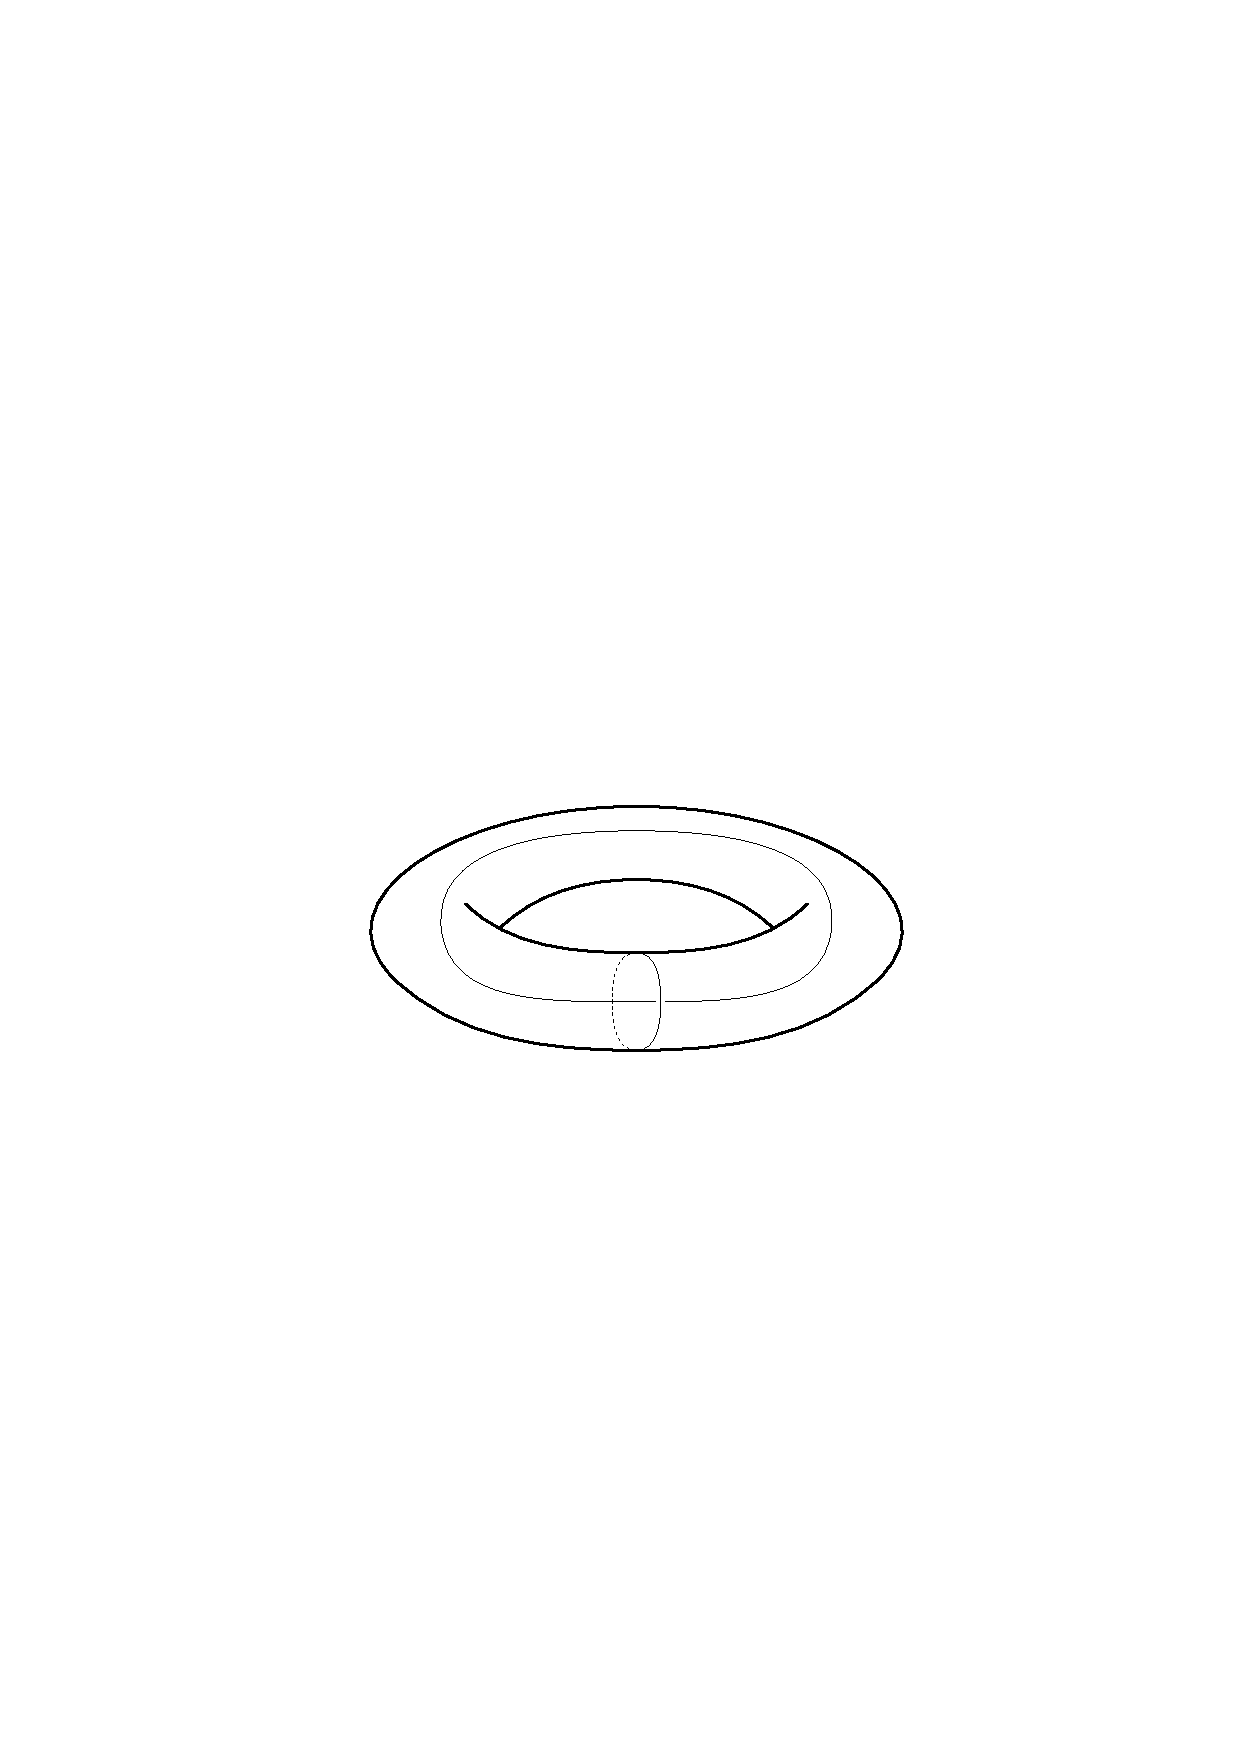
\includegraphics{chain_link_fence_knot_on_torus.pdf}
            \caption{Chain Link Fence Knot on a Torus}
            \label{fig:chain_link_fence_knot_on_torus}
        \end{figure}
        \par\hfill\par
        This last definition borrows the same difficulty from graph theory.
        While attaching handles at all of the $g$ virtual crossings yields an
        embedding into $M\times\mathbb{R}$ where $M$ is the compact orientable
        surface of genus $g$, it may have been possible to use fewer handles.
        Consider again Figs.~\ref{fig:graph_has_genus_001} and
        \ref{fig:graph_has_genus_002} where we created an embedding into the
        genus 3 compact surface. The starting graph was actually planar and
        need no additional handles (Fig.~\ref{fig:graph_has_genus_003}).
        \begin{figure}
            \centering
            \resizebox{0.5\textwidth}{!}{%
                \includegraphics{graph_has_genus_003.pdf}
            }
            \caption{Planar Embedding}
            \label{fig:graph_has_genus_003}
        \end{figure}
        \par\hfill\par
        While it is possible to compute the minimal genus of a virtual knot,
        we will not need such an algorithm. Our later work will be motivated
        by a more classical problem which is related to this difficulty.
        If one is given an extended Gauss code (a \textit{virtual knot}),
        is it possible to determine if there is a (classical) knot diagram
        that realizes this code? We can indeed do this in linear time.
        \par\hfill\par
        A valid Gauss code with $2N$ entries describes a virtual knot with
        $N$ crossings. Suppose we have embedded our virtual knot into
        $M\times\mathbb{R}$ where $M$ is a compact orientable surface of
        minimal genus. Projecting down the $\mathbb{R}$ component we obtain
        a graph embedded into $M$ where the crossings form the vertices. The
        graph is 4-valent, so by the hand-shaking theorem there are
        $2N$ edges. We are in effect decomposing $M$ into a CW complex with
        $N$ 0-cells, $2N$ 1-cells, and $F$ 2-cells. If we can compute $F$ we
        will obtain $g$ via Euler's formula:
        \begin{equation}
            V-E+F=2-2g
        \end{equation}
        Substituting $V=N$ and $E=2N$ we have:
        \begin{equation}
            g=\frac{2+N-F}{2}
        \end{equation}
        If we can compute $F$ we will have also computed $g$, and if
        $g\ne{0}$ we will know the extended Gauss code does not describe the
        knot diagram of a classical knot. We now describe how to compute $F$.
        \par\hfill\par
        \begin{figure}
            \centering
            \includegraphics{thickened_crossings.pdf}
            \caption{Signed Thickened Crossings}
            \label{fig:thickened_crossings}
        \end{figure}
        Thicken the knot projection so that the crossings look like
        Fig.~\ref{fig:thickened_crossings}. Begin traveling along the thickened
        knot, following the orientation given by the Gauss code, and place your
        finger on the left wall at all times. When you come to a crossing,
        turn left so that your finger remains continuously on the wall of the
        thickened knot. Continue doing this until you return to your starting
        point. You will have just traced out a $k$-gon for some
        $k\in\mathbb{N}$. Attach a 2-cell by gluing along this polygon.
        Continue doing this until all $4N$ of the corners of the thickened
        crossings (again, appeal to Fig.~\ref{fig:thickened_crossings}) have
        be traveled. The total number of faces, which is the total number of
        cycles you've traveled, has now been computed. We require $4N$ steps,
        and so our algorithm does indeed run in linear time.
        \par\hfill\par
        The steps described translate to jumping between the entries in the
        Gauss code in a well-defined manner. \textit{Going left} means changing
        crossing type and then walking with or against the orientation.
        That is, if you come to entry \texttt{Ons}, with \texttt{n} the index
        and \texttt{s} the sign, jump ahead to \texttt{Uns}, changing crossing
        type. You then proceed to either the next entry in the Gauss code or
        the previous entry depending on the value of the sign \texttt{s}.
        This amounts to walking forwards or backwards. The correct direction
        can be computed from Fig.~\ref{fig:thickened_crossings}. If you are at
        the final entry and need to proceed forward, loop back around to the
        start. Similarly, if you are at the starting entry and need to move
        backwards, jump ahead to the end of the Gauss code. By repeatedly
        doing this we can compute the number of cycles and consequently
        calculate the genus.
        \par\hfill\par
        Applying this algorithm to the standard 3-crossing trefoil (either the
        left handed or right handed) will yield 5 faces, giving us a genus of
        0. The chain link fence knot \texttt{O0+ U1+ U0+ O1+} produces 2 faces,
        and so we end up with a genus 1 knot diagram which can be embedded on
        the torus. The faces, and the reason for the name
        \textit{chain link fence}, can be easily seen if we conduct our drawings
        on the flat torus (Fig.~\ref{fig:chain_link_fence_knot_on_flat_torus}).
        If we lift to the universal cover of the torus, which is the Euclidean
        plane, we can see the two aforementioned faces, as well as a chain
        link fence pattern
        (Fig.~\ref{fig:chain_link_fence_knot_on_flat_torus_universal_cover}).
        \begin{figure}
            \centering
            \includegraphics{chain_link_fence_knot_on_flat_torus.pdf}
            \caption{Chain Link Fence Virtual Knot on a Flat Torus}
            \label{fig:chain_link_fence_knot_on_flat_torus}
        \end{figure}
        \begin{figure}
            \centering
            \resizebox{\textwidth}{!}{%
                \includegraphics{%
                    chain_link_fence_knot_on_flat_torus_universal_cover.pdf
                }
            }
            \caption{Lift of the Chain Link Fence to the Universal Cover}
            \label{fig:chain_link_fence_knot_on_flat_torus_universal_cover}
        \end{figure}
        \par\hfill\par
        It should be considered a pleasant bonus if a knot invariant is also
        an invariant for virtual knots. It is especially enjoyable when an
        algorithm for a knot invariant can be copied for virtual knots with
        little or no additional effort. But, before proceeding, two warnings
        are worth mentioning.
        \par\hfill\par
        The operations of the Reidemeister moves are stricter for virtual knots
        via extended Gauss code. For classical knots, should we find
        \texttt{On Om} followed by \texttt{Un Um}, or any re-ordering thereof,
        we can apply Type II and delete the four entries from the code. This is
        not so for virtual knots. Indeed, were it true the chain link fence
        would be equivalent to the unknot. The sign is crucial for a correct
        description of Type II moves in the virtual setting. For a true
        Type II move, the signs alternate. This in agreement with the fact that
        Type II does not change the writhe of a diagram. So, should we find
        \texttt{On+ Om-} followed by \texttt{Un+ Um-}, or any re-ordering
        thereof, we may apply Type II and delete the four entries, be it a
        classical or virtual knot.
        \par\hfill\par
        Lastly, the algorithm described previously computed the genus of a
        virtual knot \textit{diagram}, and not the minimal genus of all
        possible equivalent diagram. By application of Type II it is possible
        give the right-handed trefoil a genus 1 knot diagram, for example
        \texttt{O0+ U1+ O2+ O3- O4+ U0+ U3- U2+ O1+ U4+}. The Reidemeister
        moves may change the genus of a diagram.
    \subsection{Planar Diagrams}
        Planar diagram code, commonly called PD code, is one of the more popular
        representations found in programming libraries. We start with an
        oriented knot diagram and pick a starting point. We follow the
        orientation and label the \textit{arcs}, the edges between crossings,
        in increasing order from $0$ to $2N-1$ where $N$ is the number of
        crossings. Once the arcs have been labeled we once again walk around
        the knot diagram and each time we come across an under crossing we write
        down \texttt{X[a,b,c,d]} where \texttt{a} is the number of the arc you
        are coming from, \texttt{c} is the arc you'll be leaving through,
        \texttt{b} is the arc to your \textit{right}, and \texttt{d} is the
        arc to your \textit{left}. The PD code of the diagram is the ordered
        sequence of 4-tuples \texttt{X[a,b,c,d]} for each under crossing you
        encounter in the order you encounter them. Using
        Fig.~\ref{fig:trefoil_knot_arcs_labeled}, the right-handed trefoil can
        represented by writing \texttt{X[1,5,2,4],X[3,1,4,0],X[5,3,0,2]}.
        \begin{figure}
            \centering
            \includegraphics{trefoil_knot_arcs_labeled.pdf}
            \caption{Trefoil Knot with Arcs Labeled}
            \label{fig:trefoil_knot_arcs_labeled}
        \end{figure}
        \par\hfill\par
        Planar diagram code can recover unsigned Gauss code, but moreover
        the sign of the crossings can also be computed. Since the arcs are in
        increasing order, we have that for each entry
        \texttt{X[a,b,c,d]}, the difference $\texttt{c}-\texttt{a}$ is either
        1 or $1-N$, with $1-N$ occurring if and only of \texttt{a} is the final
        arc in the ordering. In contrast, the difference $\texttt{d}-\texttt{b}$
        can be $+1$ or $-1$, once reduced mod $N$. $+1$ means the crossing is
        positive and $-1$ means the crossing is negative. Whether this is a
        lucky coincidence, or if the signing of the crossings was originally
        chosen to yield this result, one must admit it is a rather elegant
        computation.
        \par\hfill\par
        Since the signs of the crossings can be computed, and since
        PD code can determine the unsigned Gauss code, we immediately see that
        PD code and extended Gauss code have the same information. Because of
        this one may use PD codes for virtual knots as well, but the phrasing
        \textit{virtual planar diagram code} is rather unfortunate for
        non-planar virtual knot diagrams. At any rate, it is \textit{not}
        common practice to use PD codes to represent virtual knots. Indeed,
        some programming libraries have checks to ensure the input PD code
        represents a planar knot diagram before allowing computations to be
        performed.
    \subsection{Dowker-Thistlethwaite Notation}
        Dowker-Thistlethwaite code (DT code for short) compactly describes
        knots. Because of this it is used in tabulation efforts where millions
        of distinct knot are listed in massive tables
        (see, for example \cite{Burton2020TheN3} and \cite{regina}).
        \par\hfill\par
        Start with an oriented knot diagram and choose a starting point.
        Walk along the knot, following the orientation, and number the
        crossings as you pass them in increasing order. For each odd number,
        if you are on the under strand as you pass the crossing,
        prepend a minus sign. Should you come upon a crossing you've already
        marked, label it again with the second number second number as well.
        At the end you should have a permutation of all numbers (with possible
        minus signs) between $0$ and $2N-1$ where $N$ is the number of
        crossings, each crossing having two numbers assigned to it. If the knot
        diagram is \textit{planar} and represents a classical knot, by a
        parity argument and the Jordan curve theorem we see that each crossing
        will have one odd number and one even number associated to it. Pair
        the numbers together into tuples $(2n,\,\pm{2m+1})$ corresponding to the
        same crossing. Lastly, order the tuples lexicographically by giving
        preference to the first entry (the even number in the tuple).
        The DT code is the corresponding ordered sequence of even numbers,
        with minus signs included.\footnote{%
            In computer science it is very common to start numbering at zero,
            which is what we have done several times throughout. In the
            original paper the labeling start at 1. Because of this the
            \textit{even} numbers are given plus and minus signs, and the
            tuples are ordered with respect to the \textit{odd} numbers. A
            minor change, but a very important one. Failure to be consistent
            can result in the wrong DT code!
        }
        \par\hfill\par
        Quite verbose, let us consider an example.
        Fig.~\ref{fig:trefoil_knot_oriented_001} depicts an oriented
        right-handed trefoil, let's start with this. Choosing the top-most
        point, we obtain the sequence of ordered tuples
        $(0,\,3)$, $(2,\,5)$, $(4,\,1)$. So our DT code for the right-handed
        trefoil is \texttt{3 5 1}. The same DT code is attainable for the
        left-handed trefoil, meaning the notation is mirror insensitive. Still,
        it is extremely compact. The following theorem further justifies its
        use.
        \begin{theorem}[Dowker, Thistlethwaite 1983]
            If two prime knots have the same DT code, then they are either
            equivalent or are mirrors of one another.
        \end{theorem}
        \begin{proof}
            See \cite{DOWKER198319}.
        \end{proof}
        Since knot tabulation rarely differentiates between mirrors, and
        almost exclusively concerns itself with the listing of prime knots,
        DT code is perfect for such an endeavor.
        \par\hfill\par
        Since the code consists entirely of odd numbers we can obtain the
        \textbf{simplified DT code} by subtracting one and dividing by two,
        doing this to each element. The trefoil then becomes
        \texttt{1 2 0}. Furthermore, should we be concerned with knots of
        no more than 26 crossings, we can substitute numbers with letters.
        This is the \textbf{alphabetical DT code}. The trefoil becomes
        \texttt{bca}. Should a minus sign be part of the original DT code
        we would add one and divide by two for the simplified code, and the
        alphabetical code would be given using a capital letter. For example,
        the knot $8_{19}$ in the Rolfsen table
        has the alphabetical DT code
        \texttt{bdFaGHCE}. In our presentation of knot tables we will
        exclusively use the alphabetical DT notation for its brevity.
    \subsection{Braids}
        Braids are one of the original means of representing knots
    \subsection{Tangles}
    \subsection{Tait Graphs}

        \section{Knot Recognition}
    Now that we have the means to represent knots, we take a brief moment to
    discuss \textit{recognizing} them. Knot theory is an extremely
    challenging field when it comes to numerical
    analysis. Many other tasks regularly enjoy polynomial time algorithms and
    highly optimized implementations. As a popular example, signal processing
    makes frequent use of the Fast Fourier Transform (FFT) which runs in
    $O\big(N\log(N)\big)$ time. Let it be known that the dreaded na\"{i}ve
    Fourier transform runs with a \textit{horrid} $O(N^{2})$ complexity.
    The inferior $O(N^{2})$ algorithm is considered completely unusable by
    those in engineering and physics.
    Professionals in other fields may then think of
    knot theorists as masochists when they hear that $O(2^{N})$ and
    $O(N!)$ algorithms are considered decent.
    \par\hfill\par
    The quintessential problem in knot theory is that of discerning two knot
    diagrams. As mentioned,
    (\cite{Reidemeister1927}, \cite{AlexanderBriggs1926}) it has been known
    since the 1920s that two knots are equivalent if and only if there is a
    finite sequence of Reidemeister moves between them. One may then ask
    \textit{how many moves are needed}?
    In \cite{HassLagarias2001} Hass and Lagarias found an
    explicit upper bound for the number of moves required to convert an
    unknot with $N$ crossings to its usual zero crossing diagram. The
    bound is $2^{cN}$ where $c$ is the constant $10^{11}$.%
    \footnote{%
        The authors remarked that this can be improved.
        For the simplest input of $N=1$ we get an upper bound of
        $2.5\times{10}^{30,102,999,566}$ Reidemeister moves,
        when only one is required.
    }
    Henrich and Kauffman were able to improve this for all \textit{reasonable}
    knot diagrams with a factorial expression. The complexity only grows
    larger than the Hass-Lagarias formula for knots with more than
    $10^{10^{10}}$ crossings \cite{HenrichKauffman2010Unknotting}. More
    recently in 2015 Lackenby discovered a polynomial bound of
    $(236N)^{11}$ \cite{Lackenby2015Unknotting}.
    \par\hfill\par
    It must be reiterated that such bounds are simply for the
    \textit{unknot}, the simplest of all knots.
    A simple algorithm for detecting if any knot diagram corresponds to the
    unknot can be made using these bounds. Loop through all possible
    combinations of Reidemeister moves of length $(236N)^{11}$ for your
    initial $N$ crossing knot diagram and if you never
    find the standard diagram for the unknot,
    then you know your original diagram
    is of a different knot type. In practice the universe will reset itself
    before your algorithm terminates when implemented on real hardware. That is,
    there are around $3^{(236N)^{11}}$ combinations of Reidemeister moves to
    check. Inputting something as small as $N=2$ yields roughly
    $10^{10^{29}}$ combinations. For comparison, the age of the universe is
    about $10^{18}$ seconds, and even if we could check, say, one million
    combinations per second, such super long time scales are starting to
    approach Poincar\'{e} recurrence.\footnote{%
        Under several assumptions for our universe.
    }
    \par\hfill\par
    Detecting the unknot requires alternative methods. One of the methods we
    will discuss in detail is \textit{Khovanov homology}, which was shown in
    2011 by Kronheimer and Mrowka to detect the unknot
    \cite{KronheimerMrowka2011KhovanovUnknot}. The na\"{i}ve algorithm runs
    like $O(\textrm{poly}(N)\cdot{2}^{N})$, which is still bad but
    significantly better than our previous $O(3^{(236N)^{11}})$ approach.
    Morever, Bar-Natan's 2006 paper provides some excellent speed boosts
    \cite{BarNatan2006FASTKH} allowing us to run the computation
    (experimentally) like $O(\textrm{poly}(N)\cdot{2}^{\sqrt{N}})$.
    \par\hfill\par
    Recognizing the unknot is still a very active area of research. In 2021
    Lackenby developed an algorithm that runs in
    $O(2^{\log(N)^{3}})$, quasi-polynomial time
    \cite{LackenBy2021QuasiPolyUnknotting}. The complexity of this problem
    has been well studied. In 2014 Kuperberg proved (assuming the generalized
    Riemann hypothesis is true) that knottedness is both \texttt{NP} and
    \texttt{co-NP} \cite{Kuperberg2014KnottednessNP}. This result has also been
    proved without the assumption of the generalized Riemann hypothesis
    \cite{Lackenby2021UnknotNP}.
    \par\hfill\par
    The more general problem of recognizing non-trivial knots is much harder.
    The number of Reidemeister moves required does have an upper bound
    \cite{CowardLackenbyReidemeisterUpperBound}, but we enter the realm of
    ridiculousness. For two knot diagrams with at most $N$ crossings, we need
    no more than $2^{2^{\cdot^{\cdot^{\cdot^{{2^{N}}}}}}}$ Reidemeister moves
    where the tower consists of a \textit{measely}
    $10^{1,000,000N}$ number of 2's. An algorithm to determine if two knot
    diagrams are of the same type can be made by looping through the
    $3^{2^{2^{\cdot^{\cdot^{\cdot^{{2^{N}}}}}}}}$ combinations of Reidemeister
    moves, but when exponentiating an integer barely changes it
    you are officially working with numbers that are too big. Indeed,
    proclaiming \textit{there exists an algorithm} almost seems fictitious.
    Does there really? There are not enough bits of memory in the observable
    universe to store such an integer, so perhaps there does not.
    \par\hfill\par
    We do not need to loop through such astronomically large combinations of
    Reidemeister moves. Hakken's \textit{normal surface theory} suffices,
    but it too consists of very difficult computational complexities
    \cite{HASS1998569}. When attempting to make tabulations of knots,
    such as the 350+ million knots in \cite{Burton2020TheN3}, we'll need
    other methods. This is where \textit{knot invariants} come in, which will
    take up the contents of the next chapter.

    \chapter{Knot Invariants}
        Distinguishing the unknot from the trefoil seems intuitively clear. To prove
such a claim becomes trivial by introducing \textit{knot invariants}, which
are mathematical objects assigned to knot diagrams that do not change under
Reidemeister moves. The knot group is perhaps the easiest to describe, given
an embedding $\gamma:\mathbb{S}^{1}\rightarrow\mathbb{R}^{3}$ we simply
compute $\pi_{1}(\mathbb{R}^{3}\setminus\gamma[\mathbb{S}^{1}])$. Since
Reidemeister moves do not change the topology of the knot complement, this is
a valid knot invariant. Computing the knot group for the unknot produces
$\mathbb{Z}$, whereas the trefoil yields a non-Abelian group with presentation
$\langle{a,\,b}\;|\;aba=bab\rangle$.
\par\hfill\par
An easier and more pictorial method exists, \textit{tricolorability}, in which
we color the arcs of a knot diagram with three colors so that all three colors
meet at the crossings, or only one color is present at a crossing. We are
required to use each color at least once. Such a notion is indeed a knot
invariant, as can be checked via the Reidemeister moves. The trefoil is
tricolorable (see Fig.~\ref{fig:trefoil_tricolor}) whereas the unknot is not.
\par\hfill\par
\begin{figure}
    \centering
    \resizebox{0.4\textwidth}{!}{%
        \includegraphics{trefoil_tricolor.pdf}
    }
    \caption{Tricoloring of the Trefoil}
    \label{fig:trefoil_tricolor}
\end{figure}
There are a myriad of other invariants that have been invented throughout the
past century, but we will be concerned with knot polynomials and homology
theories. In particular, the Alexander, Jones, and HOMFLY-PT polynomials, and
Khovanov homology and its associated Poincar\'{e} polynomial. In this chapter
we'll define these invariants and discuss algorithms for their computation.
In the final chapter we tabulate these invariants for millions of knots
using the algorithms to be discussed.

        \section{Alexander Polynomial}
    The Alexander polynomial is one of the first great invariants of knot theory.
    It is capable of distinguishing most knots with low crossing numbers and
    its computational complexity is polynomial in time. We start with a
    knot embedded into $\mathbb{R}^{3}$ and examine the knot complement.
    The fundamental group (the knot group of the knot) contains a subgroup
    isomorphic to $\mathbb{Z}$ as can be seen by wrapping a circle $n$ times
    around a small section of the knot, doing this for any $n\in\mathbb{Z}$.
    By the Galois correspondence of covering spaces
    \cite[Sec.~1.3]{HatcherAlgTop} there is an infinite cyclic cover,
    a covering space of the knot complement with fundamental group
    $\mathbb{Z}$. Following \cite[p.~53]{LickorishKnotTheory} we can be quite
    explicit. Take a Seifert surface $S\subseteq\mathbb{R}^{3}$, an embedded
    orientable surface that has the knot as its boundary, and remove a
    thickened form of it from $\mathbb{R}^{3}$. That is, we are removing
    $S\times(-1,\,1)$ from Euclidean space. The result is a manifold with
    boundary, where the boundary is two copies of $S$, label them $S_{+}$ and
    $S_{-}$. Label this space $Y$ and take infinitely many spaces $Y_{n}$,
    $n\in\mathbb{Z}$, each homeomorphic to $Y$ with homeomorphism
    $h_{n}:Y\rightarrow{Y}_{n}$. Take the disjoint union of them all and
    form the quotient space by identifying $h_{n}[S_{-}]$ with $h_{n+1}[S_{+}]$.
    The result is a covering space $X$ with fundamental group $\mathbb{Z}$
    for the knot complement. There is a Deck transformation
    $t:X\rightarrow{X}$ given by $t|Y_{n}=h_{n+1}h_{n}^{-1}$ which
    shifts the sheets by one. This acts on the first homology group
    $H_{1}(X,\,\mathbb{Z})$ allowing the group to be viewed as a
    module over $\mathbb{Z}[t,\,t^{-1}]$. This is the
    \textbf{Alexander module}. It is finitely presentable and can be
    represented by the \textbf{Alexander matrix}. If there are $r$ generators,
    we can consider the ideal generated by all $r\times{r}$ minors of the
    matrix, and this is called the \textbf{Alexander ideal}. In
    \cite{AlexanderTopologicalInvariants} it is shown such an ideal is
    principle and non-zero. Given a generator, scaling by $\pm{t}^{\pm{n}}$ will
    also be a generator. Alexander's original polynomial is the generator with
    positive constant term.
    \par\hfill\par
    A combinatorial description is given in
    \cite[p.~49]{LivingstonKnotTheory} that makes computation easier. Starting
    with an oriented knot diagram. Label the $N$ crossings and $N$ arcs
    between under crossings. That is, an arc starts at an under crossings and
    continues over all over crossings it may see until it reaches another
    under crossing. The entirety of this curve counts as one arc.
    Form an $N\times{N}$ matrix with coefficents in $\mathbb{Z}[t]$
    as follows. Travel to the end of the $\ell^{\small\textrm{th}}$ arc.
    There is an over crossing in front with the $m^{\small\textrm{th}}$
    arc passing through, and the $(\ell+1)^{\small\textrm{th}}$ arc is on the
    other side. If the crossing is positive, place $1-t$ in the
    $(n,\,\ell)$ entry, where $n$ is the number of this particular crossing,
    and $-1$ in the $(n,\,m)$ slot. For negative crossings put
    $1-t$ in $(n,\,\ell)$, $t$ in $(n,\,m)$, and
    $-1$ in $(n,\,m+1)$. Should any of the three integers $m$, $\ell$, and $m+1$
    be equal, sum the corresponding values for that entry. All other entries
    are zero. The Alexander polynomial is computed by the
    determinant of the $(N-1)\times(N-1)$ matrix formed by crossing out the
    last row and last column. Should $N-1=0$ we take the determinant to be
    one. Choice of labeling can scale the polynomial by $\pm{t}^{n}$. We thus
    define the \textbf{Alexander polynomial} $\Delta_{K}(t)$ to the result of
    the determinant shifted by $\pm{t}^{n}$ so that
    $\Delta_{K}(t)=\Delta_{K}(t^{-1})$ and so that the constant term is
    non-negative.
    \par\hfill\par
    Using sparse matrices we can fill up the matrix in $O(N)$ time. A full
    matrix where we'd be require to enter in the zero values can be rendered
    in $O(N^{2})$ time. The bulk of the computation then lies in the
    determinant. The na\"{i}ve Laplace expansion runs in $O(N!)$ time but it
    is a well-known fact in computational linear algebra that $LU$
    decomposition can be used to perform the calculation in cubic time,
    $O(N^{3})$.
    \par\hfill\par
    Being a polynomial time invariant
    it is often the first thing a knot theorist will
    compute when trying to differentiate two knots. As the number of crossings
    increases the strength seriously diminishes and it becomes more likely
    for distinct knots to have identical Alexander polynomials. Nevertheless,
    its computation is quite fast and has even been improved in recent years
    \cite{BarNatanPolynomialTimeKnotPolynomials}. The implementation used
    for tabulating the Alexander polynomial is based on this newer method.

        \section{Jones Polynomial}
    The main invariant we will be working with is the Jones polynomial. It is
    far more powerful, statistically speaking, than the Alexander polynomial
    at distinguishing knots but this comes at the cost of increased
    computational complexity. Indeed, the computation is known to be
    \textbf{NP-Hard} and the best algorithms are of $O(2^{c\sqrt{N}})$ where
    $N$ is the number of crossings and $c$ is some constant (which varies
    across algorithms). Polynomial-time quantum algorithms have been devised,
    but these have yet to see practical use.
    \subsection{The Temperley-Lieb Algebra}
        The original definition uses braids and the Temperley-Lieb algebra
        over the commutative ring $\mathbb{Z}[t,\,t^{-1}]$. For a general
        commutative ring $R$ and fixed element $\delta\in{R}$ we construct
        an $R$-algebra with generators $e_{0},\,e_{1},\,\dots,\,e_{N-2}$,
        where $N\in\mathbb{N}$ is fixed, with the following constraints:
        \begin{align}
            e_{n}^{2}&=\delta{e}_{n}
            \tag{for all $0\leq{n}\leq{N-2}$}\\
            e_{n}e_{n+1}e_{n}&=e_{n}
            \tag{for all $0\leq{n}\leq{N-3}$}\\
            e_{n}e_{n-1}e_{n}&=e_{n}
            \tag{for all $1\leq{n}\leq{N-2}$}\\
            e_{n}e_{m}&=e_{m}e_{n}
            \tag{for all $0\leq{m,n}\leq{N-2}$ with $|m-n|\geq{2}$}
        \end{align}
        The algebra is denoted $TL_{N}(\delta)$, or just $TL_{N}$ if $\delta$
        is clear from context. In the case of the Jones polynomial we choose
        $R=\mathbb{Z}[t,\,t^{-1}]$ and $\delta=-t^{2}-t^{-2}$. For any
        $N\in\mathbb{N}$ there is a group representation
        $\rho:B_{N}\rightarrow{TL}_{N}$ where the $n^{\small\textrm{th}}$
        generator $\sigma_{n}$ of $B_{N}$ is mapped to
        $te_{n}+t^{-1}\textrm{id}$, where $\textrm{id}\in{TL}_{N}$ is the
        unital element.
        \par\hfill\par
        There exists a trace operation
        $\textrm{tr}:TL_{n}\rightarrow\mathbb{Z}[t,\,t^{-1}]$ called the
        \textit{Markov trace} and the Jones polynomial of an element
        $g\in{B}_{N}$ is defined as:
        \begin{equation}
            V_{N}(g)=\delta^{N-1}\textrm{tr}\big(\rho(g)\big)
        \end{equation}
        If two words $g_{0}\in{B}_{N}$, $g_{1}\in{B}_{M}$ have isotopic
        braid closures in the plane, then their Jones polynomials will be
        identical. By Alexander's theorem every knot has a
        representative braid, and hence the Jones polynomial of the knot is
        the Jones polynomial of any such braid. Since isotopic braid closures
        yield identical polynomials, we do indeed have a knot invariant.
    \subsection{Kauffman Bracket}
        The polynomial is made pictorial, and lends itself more easily
        to computation, via the Kauffman bracket polynomial. The Jones
        polynomial can be computed by an appropriate normalization. The bracket
        polynomial is defined recursively in terms of
        \textit{smoothings} of a link diagram. Note, the definition we'll work
        with is similar to the description provided in
        \cite{BarNatan2002khovanov}. It differs slightly from the original
        \cite{KauffmanStateModels}.
        \par\hfill\par
        Resolving, or smoothing, a crossing equates to removing it.
        There are two ways to do this. Given an unoriented knot diagram
        we rotate our heads until the over crossing travels from the top left
        to the bottom right. We will label the two smoothings as the
        0-smoothing and the 1-smoothing, respectively, and these can be seen
        in Fig.~\ref{fig:resolving_crossing}. Using such binary notation has
        computational benefits, but it is also common to label these $A$ and
        $B$ smoothings.
        \begin{figure}
            \centering
            \includegraphics{resolving_crossings.pdf}
            \caption{Resolving a Crossing}
            \label{fig:resolving_crossing}
        \end{figure}
        \par\hfill\par
        For a link diagram $L$ the definition of the Kauffman bracket
        polynomial is:
        \begin{align}
            \label{eqn:kauffman_bracket}
            \langle\emptyset\rangle&=1\\
            \langle{L\sqcup\mathbb{S}^{1}}\rangle&=(q+q^{-1})\langle{L}\rangle\\
            \langle{L}\rangle&=
                \langle{L_{n,0}}\rangle-q\langle{L_{n,1}}\rangle
        \end{align}
        where $L_{n,0}$ and $L_{n,1}$ are the links obtained from the
        0 and 1 smoothings of $L$ at the $n^{th}$ crossing, respectively. The
        notation $L\sqcup\mathbb{S}^{1}$ means the disjoint union of
        $L$ with an unknot. Hence the Kauffman bracket of the
        unknot is $q+q^{-1}$.
        \par\hfill\par
        The Kauffman bracket is invariant under Type II and Type III moves.
        Type I, on the other hands, scales the polynomial by $q$ or $q^{-1}$,
        depending on the sign of the introduced crossing. Hence the Kauffman
        bracket is an invariant of \textit{framed} or \textit{regular} knots
        and links. Since scaling by a power of $q$ does not alter the individual
        coefficients for the polynomial, this finite sequence is indeed a link
        invariant. There are two ways to make an invariant polynomial out of
        this. Should the link diagram $L$ be oriented, the
        \textit{unnormalized} Jones polynomial is given by:
        \begin{equation}
            \label{eqn:unnormalized_jones}
            \tilde{J}_{L}(q)=(-1)^{N_{-}}q^{N_{+}-2N_{-}}\langle{L}\rangle
        \end{equation}
        where $N_{+}$ and $N_{-}$ are the number of positive and negative
        crossings in the diagram, respectively. This introduction of the
        crossing signs does not change under Type II and Type III, essentially
        since the write does not change, and has the added bonus of making
        $J_{L}$ invariant under Type I as well.
        \par\hfill\par
        Noticing that the defining
        equations for the Kauffman bracket imply that for any non-empty link
        diagram $L$ the bracket polynomial is divisible by $q+q^{-1}$, we
        define the \textit{normalized} Jones polynomial to be:
        \begin{equation}
            J_{L}(q)=\frac{1}{q+q^{-1}}\tilde{J}_{L}(q)
        \end{equation}
        This final polynomial is in agreement with the original braid-theoretic
        definition, though using some alternative definitions one may need to
        make the substitution $q\mapsto{q}^{1/2}$.
        \par\hfill\par
        The other, far less common, method is to scale the bracket so that
        it is a genuine polynomial, and not a Laurent polynomial. That is,
        scale the bracket by $q^{-\textrm{mindeg}(\langle{L}\rangle)}$
        ensuring that the zeroth coefficient is for the constant term. This has
        two benefits. First, it is well-defined for unoriented links, whereas
        the previous definition yields different polynomials for different
        orientations of the same link. Second, it is a genuine polynomial and
        not a Laurent polynomial. Because of this one may study the Julia set
        and Newton basin's of the associated meromorphic function
        $z\mapsto{z}-J_{L}(z)/J_{L}'(z)$, $z\in\mathbb{C}$. The topology of
        such sets are dependent only on the Jones polynomial, and
        are hence knot invariants. The Newton basins for the right-handed
        trefoil are shown in
        Fig.~\ref{fig:newton_fractal_right_trefoil_jones}.
        \par\hfill\par
        An argument for the mainstream definition is that it satisfies
        $J_{L}(q)=J_{m(L)}(q^{-1})$ where $m(L)$ is the mirror of $L$. This
        alternative definition does not.
        \begin{figure}
            \centering
            \resizebox{\textwidth}{!}{%
                \includegraphics{newton_fractal_right_trefoil_jones.png}
            }
            \caption{Newton Basins for the Right-Handed Trefoil}
            \label{fig:newton_fractal_right_trefoil_jones}
        \end{figure}
    \subsection{An Explicit Algorithm Using Gauss Code}
        The splitting operation
        $\langle{L}\rangle=\langle{L_{n,\,0}}-q\langle{L_{n,\,1}}\rangle$ at
        the $n^{\small\textrm{th}}$ crossing in a link diagram $L$ gives us a
        recursive algorithm for the computation Kauffman bracket, and hence
        the Jones polynomial. Such an algorithm is not only exponential in
        time, but exponential in space as well. Analysis of the memory
        requirements for algorithms has become increasingly rare in modern
        times since 64GB and 128GB memory is becoming increasingly
        commonplace even for personal computers, but an exponential-in-space
        algorithm will eat through this very quickly. By expanding the
        recursive definition into an iterative one we can reduce the memory
        requirements to linear. The time-complexity will still be exponential.
        \par\hfill\par
        Given a link diagram $L$ label the $N$ crossings in some way from $0$
        to $N-1$. Given any number $0\leq{n}\leq{2}^{N}-1$ we may associate a
        \textbf{complete smoothing} of the link diagram to $n$ as follows.
        Write out the number $n$ in binary. Since it falls between $0$ and
        $2^{N}-1$ this can be done using $N$ bits. If the
        $m^{\small\textrm{th}}$ bit of $n$ is zero, perform a 0-smoothing at
        the $m^{\small\textrm{th}}$ crossing. Otherwise perform a 1-smoothing.
        Every possible combination of smoothings is then uniquely represented
        by a single integer between $0$ and $2^{N}-1$.
        \par\hfill\par
        \begin{figure}
            \centering
            \includegraphics{trefoil_knot_cube_of_resolutions.pdf}
            \caption{Cube of Resolutions for the Right-Handed Trefoil}
            \label{fig:trefoil_knot_cube_of_resolutions}
        \end{figure}
        Take, for example, the right-handed trefoil in
        Fig.~\ref{fig:right_handed_trefoil_gauss_code} with the same labeling
        scheme given in the figure. There are three crossings and so we have
        $2^{3}=8$ possible resolutions. The diagram
        in Fig.~\ref{fig:trefoil_knot_cube_of_resolutions} is called the
        \textit{cube of resolutions} for the right-handed trefoil.
        This language is slightly misleading since the cube of
        resolutions is dependent on the knot diagram, so it is better to say
        this is the cube of resolutions for the standard diagram of
        the right-handed trefoil.
        \par\hfill\par
        In general, for an $N$ crossing knot, the cube of resolutions will
        generate an $N$ dimensional hypercube with a different complete
        smoothing at each vertex. The image becomes complicated very quickly
        since the size of the cube is exponential in the number of crossings.
        The cube of resolutions for the figure-eight knot is shown in
        Fig.~\ref{fig:figure_eight_knot_cube_of_resolutions}.
        Connecting the appropriate images with arrows results in the tesseract
        graph. For neatness, this has been omitted.
        \begin{figure}
            \centering
            \resizebox{\textwidth}{!}{%
                \includegraphics{figure_eight_knot_cube_of_resolutions.pdf}%
            }
            \caption{Cube of Resolutions for the Figure-Eight}
            \label{fig:figure_eight_knot_cube_of_resolutions}
        \end{figure}
        \par\hfill\par
        The third defining equation for the Kauffman bracket
        (Eqns.~\ref{eqn:kauffman_bracket})
        reduces an $N$ crossing link into two $N-1$ crossing
        links, one link obtained from the 0 smoothing, the other from the
        1 smoothing. If we continue this recursive step we'll end up with
        $2^{N}$ completely resolved links, each being the disjoint union of
        circles. Applying the first and second equations, we can inductively
        prove the following formula for the Kauffman bracket:
        \begin{equation}
            \label{eqn:kauffman_bracket}%
            \langle{L}\rangle=\sum_{n=0}^{2^{N}-1}
                (-q)^{w(n)}(q+q^{-1})^{c(n)}
        \end{equation}
        Here, $w(n)$ is the Hamming weight of $n$, the number of 1's
        that occur in the binary expansion of $n$. Recalling that an integer
        $0\leq{n}\leq{2}^{N}-1$ represents a complete smoothing of a knot,
        $c(n)$ is the number of cycles that result from the $n$ smoothing.
        \par\hfill\par
        The Hamming weight is a well-studied function and efficient methods of
        computing it are known, including constant-time algorithms if one
        restricts their attention to fixed-width integers
        (usually 32 or 64 bit).%
        \footnote{
            By \textit{constant time} on a finite set of inputs we mean the
            required \textit{human} time for an input $n=1$ is about the same
            as $n=2^{32}-1$.
        }
        A general and portable algorithm can be done in
        $\log(N)$ time as follows.
\begin{lstlisting}[style=CStyle]
unsigned int hamming_weight(unsigned int val)
{
    unsigned int result = 0U;

    while(val != 0U)
    {
        result += val & 1U;
        val = val >> 1U;
    }

    return result;
}
\end{lstlisting}
        The code \texttt{result += val \& 1U} may need explanation.
        \texttt{val \& 1U} performs a bit-wise \texttt{AND} with \texttt{val} and
        1. Since the binary representation of 1 is zero in all slots except the
        zeroth bit, \texttt{val \& 1U} is simply checking the zeroth bit of
        \texttt{val}. We add this value to \texttt{result}, ultimately giving
        us the Hamming weight. The code \texttt{val = val >> 1U} takes val and
        shifts it 1 bit to the right. So, if we had $111_{2}$ and shift it to
        the right, we'd end up with $011_{2}$. Because of this after
        \texttt{log(val)} steps \texttt{val} would be zero, exiting the
        while-loop.
        \par\hfill\par
        For the Kauffman bracket this function is used with inputs of size
        $2^{N}-1$, where $N$ is the number of crossings, so the worst-case
        time complexity at this step is $O(N)$. For example, considering the
        resolution of the right-handed trefoil
        in Fig.~\ref{fig:trefoil_knot_cube_of_resolutions} corresponding to
        $7=111_{2}$, the loop will end after 3 steps, one step for each
        crossing. The $000_{2}$ resolution exits immediately.
        \par\hfill\par
        If speed is our game we can use compiler-intrinsics, pending the
        compiler we are using. \texttt{GCC} offers the \texttt{popcount}
        function. We could write:
\begin{lstlisting}[style=CStyle]
unsigned int hamming_weight(unsigned int val)
{
    return __builtin_popcount(val);
}
\end{lstlisting}
        This will greatly improve performance, but breaks portability.
        \texttt{MSVC} users (Windows) may find the following helpful:
\begin{lstlisting}[style=CStyle]
#include <intrin.h>

unsigned int hamming_weight(unsigned int val)
{
    return __popcnt(val);
}
\end{lstlisting}
        Again, recognizing that this is not a portable solution.
        \par\hfill\par
        With the Hamming weight settled, the remaining information needed to
        compute the Kauffman bracket is the number of cycles that result from
        the $n^{th}$ smoothing ($0\leq{n}\leq{2}^{N}-1$). This section gives a
        simple algorithm using extended Gauss code. The code outlined works for
        knots, but simple extensions could be made for links. In particular, the
        algorithm works for \textit{virtual knots} and there is no restriction
        to the classical setting.
        \par\hfill\par
        \begin{figure}
            \centering
            \includegraphics{trefoil_knot_framed_001.pdf}
            \caption{Thickened Trefoil Knot}
            \label{fig:trefoil_knot_framed_001}
        \end{figure}
        We modify the algorithm for computing the virtual knot genus so that we
        may instead count the number of cycles in a complete smoothing of all
        the crossings. Once again we thicken the knot
        (like in Fig.~\ref{fig:trefoil_knot_framed_001}). Every
        crossing becomes a four-way intersection
        (Fig.~\ref{fig:thickened_crossings}), and the idea is to loop
        over the $4N$ roads in this thickened knot, $N$ being the number of
        crossings.
        \par\hfill\par
        We first examine the negative crossing. The 0 and 1
        smoothings are shown in
        Fig.~\ref{fig:thickened_negative_crossing_smoothings}. Suppose we start
        on the bottom-left road of the 0-smoothing and walk towards the
        crossing. The smoothing in the visual equates to a road block, the thick
        black line we are unable to pass through. We are thus forced to go down
        the bottom-right road. The arrow for this road is going the wrong way,
        pointing towards the crossing and we are moving away from it.
        To preserve orientation we must walk backwards. This translates as
        follows for extended Gauss code. Approaching a negative crossing from
        the bottom left road means we have approached \texttt{Un-} in
        the code reading left-to-right, \texttt{n} being the index. The
        road block tells us to go down the bottom right road, but in reverse.
        That is, look for \texttt{On-} in the code and then go
        to the \textit{previous} entry.
        This is equivalent to walking backwards. We end up at a new crossing.
        We now know the rule for approaching a crossing from the bottom left
        road for a negative crossing given the 0-smoothing. In total there are
        16 possible cases: Is the sign \texttt{+1} or \texttt{-1}, is the type
        \texttt{U} or \texttt{O}, is the smoothing $0$ or $1$,
        is the direction forwards or backwards. The
        visuals for these 16 combinations are shown in
        Fig.~\ref{fig:thickened_negative_crossing_smoothings} and
        Fig.~\ref{fig:thickened_positive_crossing_smoothings}.
        \par\hfill\par
        \begin{figure}
            \centering
            \includegraphics{thickened_crossings.pdf}
            \caption{Signed Crossings in a Framed Knot}
            \label{fig:thickened_crossings}
        \end{figure}
        \begin{figure}
            \centering
            \includegraphics{thickened_negative_crossing_smoothings.pdf}
            \caption{Smoothing a Negative Crossing in a Framed Knot}
            \label{fig:thickened_negative_crossing_smoothings}
        \end{figure}
        \begin{figure}
            \centering
            \includegraphics{thickened_positive_crossing_smoothings.pdf}
            \caption{Smoothing a Positive Crossing in a Framed Knot}
            \label{fig:thickened_positive_crossing_smoothings}
        \end{figure}
        Jumping from the over-crossing to the under-crossing, and vice-verse,
        as is needed in the algorithm is made easier if we have an array
        \texttt{ind} such that \texttt{ind[n]} is an ordered pair whose
        zeroth entry is the index of the under-crossing for the
        $n^{\small\textrm{th}}$ crossing, and first entry is the index of the
        over-crossing. It is then
        useful to describe a \texttt{struct} for this ordered pair, and an
        algorithm to obtain this array.
\begin{lstlisting}[style=CStyle]
struct crossing_indices {
    unsigned int under;
    unsigned int over;
};

struct crossing_indices *get_indices(const struct knot *K)
{
    unsigned int n;
    struct crossing_indices *ind;

    if (!K)
        return NULL;

    if (K->number_of_crossings == 0U)
        return NULL;

    ind = malloc(sizeof(*ind) * K->number_of_crossings);

    if (!ind)
        return NULL;

    for (n = 0U; n < 2U * K->number_of_crossings; ++n)
    {
        if (K->type[n] == over_crossing)
            ind[K->crossing_number[n]].over = n;
        else
            ind[K->crossing_number[n]].under = n;
    }

    return ind;
}
\end{lstlisting}
        The error checks are for good programming practice: Check if your
        input pointer is \texttt{NULL}, don't assume \texttt{malloc} was
        successful, and don't pass zero to \texttt{malloc}. The actual algorithm
        is contained in the for loop. We loop over the Gauss code, ask which
        crossing number we have, and then add this index to our array. The
        loop requires $2N$ steps, $N$ being the number of crossings, so this
        step is $O(N)$. Unlike the Hamming weight and the number of circles
        from a resolution, this index-finding algorithm is only needed once. We
        execute the algorithm at the start and then store the result in
        memory.
        \begin{figure}
            \centering
            \includegraphics{thickened_crossing_labeled.pdf}
            \caption{Thickened Crossings with Labels}
            \label{fig:thickened_crossings_labeled}
        \end{figure}
        \begin{figure}
            \centering
            \includegraphics{thickened_crossings_resolved_labeled.pdf}
            \caption{Thickened Resolved Crossings with Labels}
            \label{fig:thickened_crossings_resolved_labeled}
        \end{figure}
        \par\hfill\par
        Because of the 16 possibilities, the full algorithm is lengthy. To make
        this easier we label the roads so that we can make a table. This is
        done in Fig.~\ref{fig:thickened_crossings_labeled} and we call this the
        \textit{road number}. By examining
        Fig.~\ref{fig:thickened_crossings_resolved_labeled} we can tell where
        we need to go as we walk along the knot. This is done explicitly in
        Tab.~\ref{tab:circle_counting_algorithm_where_go}.
        The table reads as follows.
        The left \textit{In} column tells you which road you are approaching the
        crossing from. Note if you are approaching from roads 0 or 1, you are
        walking forward, and if you are approaching from roads 2 or 3, you are
        walking backwards. Using the information about the sign and resolution
        of the crossing you know which road to leave from. In the Gauss code
        if you approach an under crossing, find the corresponding over crossing
        in the code (and vice-versa). Then go to the previous entry if you are
        leaving from roads 0 and 1, and the next entry if leaving from roads
        2 or 3. Eventually you will return to an entry in
        the Gauss code you have already been to. This amounts to 1 cycle from
        the resolution. Move on to the next element of the Gauss code you have
        yet to encounter and repeat.
        \begin{table}
            \centering
            \begin{tabular}{c c c c}
                In&Sign&Resolution&Out\\
                \hline
                0&-&0&1\\
                0&-&1&3\\
                0&+&0&3\\
                0&+&1&1\\
                \hline
                1&-&0&0\\
                1&-&1&2\\
                1&+&0&2\\
                1&+&1&0\\
                \hline
                2&-&0&3\\
                2&-&1&1\\
                2&+&0&1\\
                2&+&1&3\\
                \hline
                3&-&0&2\\
                3&-&1&0\\
                3&+&0&0\\
                3&+&1&2
            \end{tabular}
            \caption{The Circle Counting Algorithm - Where to Go}
            \label{tab:circle_counting_algorithm_where_go}
        \end{table}
        Tab.~\ref{tab:circle_counting_algorithm_where_start}
        then tells which road number you are entering based on the sign and type
        of the crossing, and the direction you are walking. Eventually the code
        will be exhausted, and the resulting tally is the number of
        circles from this resolution.
        \par\hfill\par
        \begin{table}
            \centering
            \begin{tabular}{c c c c}
                Type&Sign&Direction&In\\
                \hline
                $O$&-&Forward&1\\
                $O$&-&Backward&3\\
                $O$&+&Forward&0\\
                $O$&+&Backward&2\\
                \hline
                $U$&-&Forward&0\\
                $U$&-&Backward&2\\
                $U$&+&Forward&1\\
                $U$&+&Backward&3
            \end{tabular}
            \caption{The Circle Counting Algorithm - Where to Start}
            \label{tab:circle_counting_algorithm_where_start}
        \end{table}
        We now give the full details of the algorithm as a
        (semi) literate program. Since we are using all
        numbers between 0 and $2^{N}-1$ to describe complete resolutions of the
        knot the intermediate step must be performed with (at least) $N$-bit
        wide integers. Since the width of \texttt{int} is usually 32-bits, we
        restrict ourselves to knots with less than 32 crossings. If we change
        all of our types to \texttt{long} we can increase this to 64 crossings.
        We define \texttt{MAX\_CROSSINGS} to be either 32 or 64, pending size
        of the integers we are using.
        \par\hfill\par
        We create a buffer that is \texttt{4*MAX\_CROSSINGS} long to keep track
        of which roads we have visited. Our code starts as follows.
        \newpage
\begin{lstlisting}[style=CStyle]
unsigned int
circle_count(const struct knot *K,
             const struct crossing_indices *ind,
             unsigned int resolution)
{
    unsigned int n, number_of_circles, road_index;
    unsigned int crossing, code_index;
    unsigned char direction, crossing_resolution, road_number;
    enum crossing_sign sign;

    unsigned char have_visited[4U * MAX_CROSSINGS];

    const unsigned char forward = 0x00U;

    /* Empty knot, no cycles. */
    if (!K)
        return 0U;

    /* Unknot, 1 cycle. */
    if (K->number_of_crossings == 0U)
        return 1U;

    /* Invalid input, return 0. */
    if (!ind)
        return 0U;

    /* Initialze the buffer to have zero entries. */
    for (n = 0U; n < 4U * K->number_of_crossings; ++n)
        have_visited[n] = 0x00U;

    /* Initialize count to zero. */
    number_of_circles = 0U;
\end{lstlisting}
        with all variables and arrays initialized we start the bulk of the
        algorithm and count the number of cycles corresponding to the given
        resolution. We loop over the $4N$ roads in our thickened knot.
\begin{lstlisting}[style=CStyle, firstnumber = 34]
    for (n = 0U; n < 4U*K->number_of_crossings; ++n)
    {
        /* If we've already checked this road skip it. */
        if (have_visited[n])
            continue;
\end{lstlisting}
        Now we need the crossing index, sign of the crossing, and the road
        number (between 0 and 3). All of this can be obtained from the road
        index, which is the dummy variable \texttt{n}. This road index is
        $\texttt{n=4c+r}$ where \texttt{c} is the crossing index and
        \texttt{r} is the road number. We compute \texttt{c} by shifting
        \texttt{n} down by two bits, and we compute \texttt{r} via
        \texttt{r=n mod 4}. This yields the following:
\begin{lstlisting}[style=CStyle, firstnumber = 40]
        road_index = n;
        crossing = road_index >> 2U;
        road_number = road_index & 0x03U;
\end{lstlisting}
        Since the sign does not change between occurences of a crossing, we can
        grab the sign from either the over or under crossing entry of the Gauss
        code. We use the crossing table \texttt{ind} that we've already computed
        to aid us.
\begin{lstlisting}[style=CStyle, firstnumber = 44]
        sign = K->sign[ind[crossing].over];
\end{lstlisting}
        Lastly we need the direction we are travelling, either forwards or
        backwards. We set \texttt{forward = 0}, and so have implicitly
        declared \texttt{backward = 1}. This has the following advantage. By
        examining Fig.~\ref{fig:thickened_crossings_labeled} we see that the
        forward direction corresponds to road number 0 and 1, and backwards
        corresponds to 2 and 3. That is, the direction is determine by the
        2's bit in the road number. We compute the direction via:
\begin{lstlisting}[style=CStyle, firstnumber = 46]
        direction = road_number >> 1U;
\end{lstlisting}
        The last bit of information we need is the location of the entry in the
        Gauss code. This will be called the \textit{code index}. It can be
        computed by examining the figures above. We have:
\begin{lstlisting}[style=CStyle, firstnumber = 48]
        if (sign == positive_crossing)
        {
            if (road_number & 0x01U)
                code_index = ind[crossing].under;
            else
                code_index = ind[crossing].over;
        }

        else
        {
            if (road_number & 0x01U)
                code_index = ind[crossing].over;
            else
                code_index = ind[crossing].under;
        }
\end{lstlisting}
        We now loop over all of the roads and compute the number of cycles. We
        start with:
\begin{lstlisting}[style=CStyle, firstnumber = 64]
        while (!have_visited[road_index])
        {
            have_visited[road_index] = 0x01U;

            /* How to smooth the mth crossing. Get the mth bit. */
            crossing_resolution = (resolution >> crossing) & 0x01U;
\end{lstlisting}
        Now we need to know which road to leave on. We appeal to
        Tab.~\ref{tab:circle_counting_algorithm_where_go}. We convert this table
        into a more algebraic expression as follows. We see from
        Fig.~\ref{fig:thickened_positive_crossing_smoothings} that if we have a
        positive crossing with a 0 smoothing, then
        $0\mapsto{3}$, $1\mapsto{2}$, $2\mapsto{1}$, and $3\mapsto{0}$. We note
        that this is described by $y=3-x$. Similarly, for a 1 smoothing we have
        $0\mapsto{1}$, $1\mapsto{0}$, $2\mapsto{3}$, and $3\mapsto{2}$. This
        is described by $y=(5-x)\textrm{ mod }4$. Negative crossings may be
        handled by mirroring this. We obtain:
        \newpage
\begin{lstlisting}[style=CStyle, firstnumber = 71]
            if (sign == positive_crossing)
            {
                if (crossing_resolution == 0x00U)
                    road_number = 3U - road_number;

                else
                {
                    road_number = (5U - road_number) & 0x03U;
                    direction = 0x01U - direction;
                }
            }

            else
            {
                if (crossing_resolution == 0x00U)
                {
                    road_number = (5U - road_number) & 0x03U;
                    direction = 0x01U - direction;
                }

                else
                    road_number = 3U - road_number;
            }

            have_visited[4U*crossing + road_number] = 0x01U;
\end{lstlisting}
        Changing which road we're on means we've changed the strand we're on.
        Over goes to under and under goes to over. We need to update this by
        going to the correct entry in the Gauss code.
\begin{lstlisting}[style=CStyle, firstnumber=97]
            if (K->type[code_index] == over_crossing)
                code_index = ind[crossing].under;
            else
                code_index = ind[crossing].over;
\end{lstlisting}
        We now move along to the new entry in the Gauss code by moving either
        forwards or backwards, pending our current direction. If we're at the
        final entry in the Gauss code and are moving forward, we loop back
        around to the start. Similarly if we're at the first entry and a walking
        backwards we loop around to the final entry. This gives us:
        \newpage
\begin{lstlisting}[style=CStyle, firstnumber=102]
            if (direction == forward)
            {
                if (code_index == 2U*K->number_of_crossings - 1U)
                    code_index = 0U;
                else
                    ++code_index;
            }

            else
            {
                if (code_index == 0U)
                    code_index = 2U*K->number_of_crossings - 1U;
                else
                    --code_index;
            }
\end{lstlisting}
        Nearly done, we're now at the next entry in the Gauss code, we just need
        to know which road we're entering from. We use
        Tab.~\ref{tab:circle_counting_algorithm_where_start} for this.
\begin{lstlisting}[style=CStyle, firstnumber = 118]
            if (K->sign[code_index] == positive_crossing)
            {
                if (K->type[code_index] == over_crossing)
                {
                    if (direction == forward)
                        road_number = 0U;
                    else
                        road_number = 2U;
                }

                else
                {
                    if (direction == forward)
                        road_number = 1U;
                    else
                        road_number = 3U;
                }
            }

            else
            {
                if (K->type[code_index] == over_crossing)
                {
                    if (direction == forward)
                        road_number = 1U;
                    else
                        road_number = 3U;
                }

                else
                {
                    if (direction == forward)
                        road_number = 0U;
                    else
                        road_number = 2U;
                }
            }
        }
\end{lstlisting}
        As a slight reduction in code size, these nested conditionals can be
        replaced by an algebraic expression in our search of the
        \textit{in} road. We first note that the negative and positive crossings
        have mirrored conditional statements. We search for four variables
        $a,b,c,d$ such that:
        \begin{equation}
            r=ast+bs+ct+d
        \end{equation}
        where $r$ is the road number, $s$ is the sign, and $t$ is the type.
        Since the sign $s$ and type $t$ are represented by \texttt{enum} data
        types we may treat them as integers and add them.
        Tab.~\ref{tab:circle_counting_algorithm_where_start} tells gives us
        $a=-2$, $b=1$, $c=1$, and $d=2\cdot\texttt{dir}$, where \texttt{dir} is
        the direction ($\texttt{forward}=0$, $\texttt{backward}=1$). We can
        compute the output road number via:
\begin{lstlisting}[style=CStyle]
unsigned char
get_road_number(const struct knot *K,
                unsigned int code_index,
                unsigned char direction)
{
    const unsigned char b = K->sign[code_index];
    const unsigned char c = K->type[code_index];
    const unsigned char a = (b * c) << 1U;
    const unsigned char d = direction << 1U;
    return b + c + d - a;
}
\end{lstlisting}
        Regardless of preference (nested conditional or algebraic expressions)
        we now know which road we are entering the crossing from.
        We now update our variables and go back to the top of the
        \texttt{while} loop and continue until
        we encounter a road we've already traveled on. Once this occurs we
        increment the circle count. We do this until all $4N$ entries of the
        \texttt{have\_visited} table are set to 1. At this point the
        \texttt{for} loop will exit. We return the count and exit the function.
\begin{lstlisting}[style=CStyle, firstnumber = 157]
            crossing = K->crossing_number[code_index];
            sign = K->sign[code_index];
            road_index = (crossing << 2U) + road_number;
        }

        ++number_of_circles;
    }

    return number_of_circles;
}
\end{lstlisting}
        Let's use the trefoil as an example. The $000_{2}$ resolution results
        in 2 cycles (Fig.~\ref{fig:trefoil_knot_cube_of_resolutions}). Let's
        check that the algorithm detects this. The Gauss code is
        \texttt{O0+ U1+ O2+ U0+ O1+ U2+}.
        We start by entering the zeroth crossing
        (road 0). It is an over crossing, so we look ahead in the code and
        find the corresponding under crossing. It is a positive crossing with
        the zero resolution, so
        Tab.~\ref{tab:circle_counting_algorithm_where_go} tells
        us to leave through road 3. We mark road 0 and road 3 of the zeroth
        crossing as traveled and proceed. Leaving through road 3 means we
        travel forward. Hence we wind up at \texttt{O1+} in the code and we are
        walking forwards. Over-crossing, positive sign, walking forwards means
        we are entering the crossing from road 0
        (Tab.~\ref{tab:circle_counting_algorithm_where_start}). We will again
        leave through road 3 and enter the \texttt{O2+}
        crossing walking forwards. We again enter road 0 and leave
        through road 3 and wind up at \texttt{O0+} walking forward,
        completing our first cycle. The next untouched
        road is road 1 for the zeroth crossing. This corresponding to
        \texttt{U0+} walking forwards.
        Tab.~\ref{tab:circle_counting_algorithm_where_go}
        tells us to leave through road 2. We end up at \texttt{U1+}, road 1.
        Again we leave through road 2 and end up at \texttt{U2+} road 1.
        We leave through road 2 entering $U0+$, completing our cycle.
        All of the roads have been marked, and we have 2 cycles total,
        in agreement with Fig.~\ref{fig:trefoil_knot_cube_of_resolutions}.
        \par\hfill\par
        To compute the Kauffman bracket we loop over all integers
        $0\leq{n}\leq{2}^{N}-1$, $N$ being the number of crossings, compute the
        number of circles corresponding to the $n^{\small\textrm{th}}$
        resolution using this
        algorithm, and perform the sum in Eqn.~\ref{eqn:kauffman_bracket}. The
        circle counting algorithm requires $4N$ steps since we loop over the
        $4N$ roads, and the Hamming weight has worst-case complexity $O(N)$,
        meaning each stage is $O(4N)+O(N)=O(N)$ in time complexity. There are
        $2^{N}$ total steps, so $O(N2^{N})$ is the total complexity of the
        computation. The computation of the array of indices at the beginning
        is $O(N)$, but as mentioned is only required once and is not part of
        the inner for-loop. The result for the entire algorithm is
        $O(N+N2^{N})=O(N2^{N})$. The primary benefit here is that the space
        requirement is linear, only storing the $4N$ array of Booleans in
        memory and the Laurent polynomial itself (which is $O(N)$ in length).
        The algorithm also operates on any valid extended Gauss code, meaning
        we can use it to compute the Kauffman bracket of virtual knots.
        \par\hfill\par
        To obtain the unnormalized Jones polynomial we need to shift
        the degree of the resulting Kauffman bracket polynomial
        (Eqn.~\ref{eqn:unnormalized_jones}). The computation of $N_{-}$ and
        $N_{+}$ is $O(N)$, loop through the Gauss code and count.
        We represent Laurent polynomials by the following struct:
        \begin{lstlisting}[style=CStyle, gobble=12]
            struct laurent_polynomial {
                signed int lowest_degree;
                signed int highest_degree;
                signed int *coeffs;
            };
        \end{lstlisting}
        Once $N_{-}$ and $N_{+}$ have been computed,
        multiplication by $q^{N_{+}-2N_{-}}$ thus takes $O(1)$ in time, we
        simply add $N_{+}-2N_{-}$ to \texttt{highest\_degree} and
        \texttt{lowest\_degree}. This step does not impact the computation time
        in any significant way. A full implementation by the author is
        available as free software under the GPLv3 license
        \cite{MaguireJones}.
    \subsection{Symbolic Calculus}
        Another method of computation is worth noting since its modification
        will be used to compute Khovanov homology
        (as in \cite{BarNatan2006FASTKH}). This method is outlined in
        \cite{KatlasJones} and is the implementation used by the
        \texttt{Mathematica} package \texttt{KnotTheory`}. The algorithm
        can be modified to general programming languages lacking symbolic
        manipulations using doubly linked lists \cite{MaguireJones}.
        \par\hfill\par
        The computation begins by examining how smoothing a crossing modifies
        the PD code of a knot. The algorithm can work for link diagrams too
        where we consider sequences of PD codes, one for each component of the
        link.
        \begin{figure}
            \centering
            \includegraphics{resolving_crossings_pd_label.pdf}
            \caption{Resolving a Labeled Crossing}
            \label{fig:resolving_crossings_pd_label}
        \end{figure}
        The Kauffman relation tells us to replace ordered quadruples
        \texttt{X[a,b,c,d]} with ordered pairs
        \texttt{P[a,b]P[c,d]-$q$P[a,d]P[b,c]}
        (Fig.~\ref{fig:resolving_crossings_pd_label}).
        Gathering these \textit{affine combinations}
        at each crossing gives us a product:
        \begin{equation}
            \langle{K}\rangle
            =\prod_{n=0}^{N-1}(
                \texttt{P[an,bn]P[cn,dn]-$q$P[an,dn]P[bc,cn]}
            )
        \end{equation}
        where \texttt{X[an,bn,cn,dn]} is the
        $n^{\small\textrm{th}}$ entry in the PD code. You might think
        \textit{hey, that is linear}! Indeed, we have the product of
        $N$ affine terms, but expanding this product out into a polynomial
        will require $2^{N}$ monomial products. This expansion will be
        necessary in order to retrieve integer coefficients from our formal
        polynomial with (products of) ordered pair coefficients.
        \par\hfill\par
        Expanding the product we will obtain a polynomial where the coefficients
        are formal products of ordered pairs. The ordering of the product
        does not matter, we can take it to be commutative. Should we find a
        product of the form \texttt{P[a,b]P[b,c]} the PD code is telling us
        the \texttt{a} arc is now connected to the \texttt{b} arc after we've
        resolved the crossings, and similar that the \texttt{b} arc is
        connected to the \texttt{c} arc. \texttt{b} is now redundant and we
        may replace this with \texttt{P[a,c]}. That is, we make the formal
        substitution $\texttt{P[a,b]P[b,c]}\mapsto\texttt{P[a,c]}$. Similar
        \texttt{P[a,b]P[a,b]} tells us \texttt{a} and \texttt{b} are forming a
        cycle. We may substitute $\texttt{P[a,b]P[a,b]}\mapsto\texttt{P[a,a]}$.
        In both of the substitutions the ordering of the pairs is immaterial.
        We simply wish to know which arcs are now connected to which.
        \texttt{P[a,a]} tells us we have a loop. The Kauffman bracket says
        we replace $\texttt{P[a,a]}\mapsto{q}+q^{-1}$.
        \par\hfill\par
        If symbolic manipulations are available to you this defines a very
        compact algorithm.\footnote{%
            \cite{KatlasJones} implements this in three lines.
        }
        As mentioned, in a general programming language we can mimic these
        formal Laurent polynomial using doubly linked lists where the elements
        of the linked list are used to represent formula products of ordered
        pairs. A full implementation is provided, again under the GPLv3
        license, in \cite{MaguireJones}.
        \par\hfill\par
        The computational complexity in both time and space are on par with the
        previous Gauss code algorithm, though the actual time comparisons show
        the former method is a bit faster. Nevertheless we can modify this
        idea slightly and achieve a remarkable speed boost.
        \par\hfill\par
        Repeat the previous algorithm by picking some element in the PD code
        and undergoing the formal substitution
        $\texttt{X[a,b,c,d]}\mapsto\texttt{P[a,b]P[c,d]-$q$P[a,d]P[b,c]}$.
        Rather than doing this for each crossing,
        forming a product of affine terms,
        and then expanding, instead find the entry in the PD code with the
        \textit{most} number of elements in common with our starting one.
        That is, the entry \texttt{X[e,f,g,h]} with the highest number of
        matching integers in \texttt{X[a,b,c,d]}. We take this PD code entry
        and expand it using
        $\texttt{X[e,f,g,h]}\mapsto\texttt{P[e,f]P[g,h]-$q$P[e,h]P[f,g]}$. We
        then simplify the product
        \begin{equation}
            \nonumber
            (\texttt{P[a,b]P[c,d]-qP[a,d]P[b,c]})
            (\texttt{P[e,f]P[g,h]-qP[e,h]P[f,g]})
        \end{equation}
        using the rules before for substituting formal products of ordered
        pairs. Once simplified we add the entry in the next PD code with the
        highest number of matching entries among
        \texttt{a,b,c,d,e,f,g,h}. We continue doing this until all entries in
        the PD code have been added.
        \par\hfill\par
        We can envision this modification as follows. We pick a crossing in
        the diagram and draw a small circle around it. We find the next
        crossing with the highest number of strands going into this circle.
        We add this crossing, and enlarge our circle into a blob the engulfs
        both crossings. We then find the next crossing with the largest number
        of strands going into our blob, and enrich the blob by adding this
        crossing. The blob is our \textit{computational front}, and by
        adding the crossing with the highest number of strands in the blob we
        are increasing the size of the blob minimally. We are effectively
        ensuring we do as little simplifying as possible in our final
        expansion.
        \par\hfill\par
        While simple enough to describe, this modification of the symbolic
        calculus yields significant improvements in computational time (the
        complexity is about the same). It is not uncommon to find the
        computation is about 100x faster with this trick. On a more somber
        note, 100x faster for an exponential-like algorithm means you can
        increase the crossing number by 7 or 8 before you're back to similar
        times.
        \subsection{Tait Graph Expansion}
            The next method of computation has two uses for us. Firstly, it is
            very efficient in terms of speed, and secondly it will give us an
            explicit formula for the Jones polynomial of \textit{twist knots}.
            Later on we will appeal to this formula for calculations
            involving twist of over 90 crossings. The exponential nature of
            the algorithms we've thus far presented would otherwise prevent us
            from doing this.
            \par\hfill\par
            We appeal to the Tait graph. Given an oriented knot or link diagram
            the smoothing operations for the Kauffman bracket can translate to
            operations on the Tait graph.
        %\subsection{Torus and Twist Knots}

        \section{Khovanov Homology}
    The next invariant up is the one we're most concerned with.
    \textbf{Khovanov homology} is a link invariant that generalizes the
    Jones polynomial by \textit{categorifying} it. The concept was invented by
    Mikhail Khovanov in \cite{Khovanov1999CatJonesPoly} but we will be
    following the styling of \cite{BarNatanKhovanovJones} more closely.
    \par\hfill\par
    We start with the Kauffman relations, but instead of attaching polynomials
    to our diagram we use chain complexes. The \textit{Khovanov} bracket of a
    link diagram $L$ is given recursively via smoothings. We define
    \begin{align}
        [[\emptyset]]&=0\rightarrow\mathbb{Z}\rightarrow{0}\\
        [[\mathbb{S}^{1}\sqcup{L}]]&=V\otimes[[L]]\\
        [[L]]&=\mathcal{F}
        \big(
            0\rightarrow[[L_{n,\,0}]]\rightarrow[[L_{n,\,1}]]\{1\}\rightarrow{0}
        \big)
    \end{align}
    where $V$ is a graded vector space,
    or more generally a free $\mathbb{Z}[q]$
    module of rank two with generators of degree $+1$ and $-1$
    \cite[p.~362]{Khovanov1999CatJonesPoly}, and where
    $\mathcal{F}$ is the \textit{flatten} operation that converts a
    double chain complex into a single chain complex by taking direct sums
    of the components along the diagonals \cite[p.~338]{BarNatanKhovanovJones}.
    The $\{1\}$ notation indicates the degree shift operation which shifts the
    grading by $1$. Explicitly, if we have decomposed $V$ into
    $V=\oplus_{n}V_{n}$, then $V\{1\}_{n}=V_{n-1}$ so that the graded dimension
    of $V\{1\}$ is $q$ times the graded dimension of $V$.
    \par\hfill\par
    The last ingrediant is the differential between $[[L_{n,\,0}]]$ and
    $[[L_{n,\,1}]]\{1\}$. This is also defined pictorially. We use the cube of
    resolutions of the knot or link diagram, for example
    Fig.~\ref{fig:trefoil_knot_cube_of_resolutions}. Recalling our previous
    binary notation, every complete smoothing corresponds uniquely to a string
    of length $N$ with entries in $\{\,0,\,1\,\}$ where $N$ is the number of
    crossings in the diagram. If two strings differ in only one place then
    there is an edge between them in the cube of resolutions.
    The edge describes a cobordism
    (a pair of pants) that either fuses two cycles into one or splits a cycle
    into two. Re-examining Fig.~\ref{fig:trefoil_knot_cube_of_resolutions} is
    strongly encouraged here. Fusing amounts to a homomorphism between
    $V\otimes{V}$ and $V$, whereas splitting needs a map from
    $V$ to $V\otimes{V}$. For generators $v_{-},\,v_{+}$ of $V$ we define
    $m:V\otimes{V}\rightarrow{V}$ to be the linear function induced by:
    \begin{align}
        m(v_{-}\otimes{v}_{-})&=\mathbf{0}\\
        m(v_{-}\otimes{v}_{+})&=v_{-}\\
        m(v_{+}\otimes{v}_{-})&=v_{-}\\
        m(v_{+}\otimes{v}_{+})&=v_{+}
    \end{align}
    and define $\Delta:V\rightarrow{V}\otimes{V}$ via
    \begin{align}
            \Delta(v_{-})&=v_{-}\otimes{v}_{-}\\
            \Delta(v_{+})&=v_{+}\otimes{v}_{-}+v_{-}\otimes{v}_{+}
    \end{align}
    See \cite[p.~343]{BarNatanKhovanovJones} for further details. The
    differential is defined by an alternating sum of such maps over edges whose
    strings yield the same Hamming weight (sum of the entries in the string).
    \par\hfill\par
    By construction the Khovanov homology of a link contains the Jones
    polynomial. The Poincar\'{e} polynomial of the homology is defined by
    throwing away the torsion bits. We write
    \begin{equation}
        \label{eqn:khovanov_polynomial}
        Kh_{L}(q,t)=
        \sum_{r,\ell}t^{r}q^{\ell}\textrm{dim}\big(Kh_{\ell}^{r}(L)\big)
    \end{equation}
    where we are writing the $r^{\small\textrm{th}}$ homology group
    $Kh^{r}(L)$ as the direct sum of homogeneous components
    $Kh_{\ell}^{r}(L)$ \cite{KatlasKhoHo}.
    The Jones polynomial is recovered as the graded Euler characteristic, or
    more explicitly
    \begin{equation}
        J_{L}(q)=Kh_{L}(q,-1)
    \end{equation}
    This invariant is quite strong, but computationally expensive. This cost
    will be our greatest detriment in our work so when possible we first
    attempt to use the Jones polynomial. If this fails at differentiating
    two knots or links we then try to compute Khovanov homology or the
    \textbf{Khovanov polynomial}, which is the Poincar\'{e} polynomial of
    Khovanov homology (Eqn.~\ref{eqn:khovanov_polynomial}).
    \par\hfill\par
    The invariant is indeed stronger than the Jones polynomial and can
    distinguish quite a few more knots, though it is not a perfect
    invariant \cite{Watson2007KnotsWI}. That is, there are
    distinct knots with the same Khovanov homology, but it is a powerful
    invariant and is capable of detecting certain knot types.
    \begin{theorem}[Kronheimer and Mrowka, 2011]
        If a knot $K$ has the same Khovanov homology as the unknot, then $K$
        is equivalent to the unknot.
    \end{theorem}
    \begin{proof}
        \cite{KronheimerMrowka2011KhovanovUnknot}.
    \end{proof}
    As discussed, something as simple as determining if a diagram represents
    the unknot can require super exponential algorithms if we rely on
    Reidemeister moves alone. The definition of Khovanov homology produces a
    straight-forward algorithm that runs in $O(2^{N})$ time, albeit with
    substantially more overhead than the Jones polynomial. Combining the
    previous theorem gives a considerably more efficient algorithm of
    unknot detection than randomly looping through Reidemeister combinations.
    \par\hfill\par
    Since the Khovanov polynomial is a generalization of
    the Jones polynomial it has been conjectured that if a
    knot has the same Jones polynomial as the unknot, then that knot is
    equivalent to the unknot. At the time of this writing it has not been
    proven, but there is evidence for and against the claim.
    Thistlewaite found links with the same Jones polynomial as the unlink
    \cite{Thistlethwaite2001LINKSWT}, and there is a 3-crossing virtual
    knot that has the same Jones polynomial as the unknot. For the claim,
    all knots of up to 24 crossings are either the unknot, or have a
    Jones polynomial different from the unknot
    \cite{VerificationUnknotJonesConjUpTo24}.
    \par\hfill\par
    The numerical results in this work are motivated by the following two
    theorems.
    \begin{theorem}[Baldwin and Sivek, 2022]
        If a knot $K$ has the same Khovanov homology as either of the
        trefoils, then $K$ is equivalent to one of them.
    \end{theorem}
    \begin{theorem}[Baldwin, Dowlin, Levine, Lidman, and Sazdanovic, 2021]
        If a knot $K$ has the same Khovanov homology as the figure-eight
        knot, then $K$ is equivalent to it.
    \end{theorem}
    See \cite{BaldwinSivekKhovanovTrefoils} and
    \cite{BaldwinDowlinKhovanovFigureEight}, respectively.
    \par\hfill\par
    As mentioned the definitions provides a fairly straight-forward means of
    implementing an algorithm. This has been done in
    \cite{sage}. Unfortunately for 14 crossing knots it requires over
    100GB of data and days of computation for a single knot. 17 crossings
    knots are unapproachable my such methods. Modification of the
    symbolic calculus trick for the Jones polynomial can be performed for
    Khovanov homology \cite{BarNatan2006FASTKH} and with this we can
    remarkably compute with 60 crossing knots in about a day on modern hardware.

        \section{HOMFLY-PT Polynomial}
    The last invariant we'll investigate is the HOMFLY-PT polynomial, which
    contains both the Alexander and Jones polynomials in it. Like the Jones
    polynomial it is defined via skein relations where we smooth crossings.
    Given a link diagram $L$ define $L_{n,\,0}$ to be the 0-smoothing of the
    $n^{\small\textrm{th}}$ crossing and $L_{n,\,\textrm{flip}}$ to be the
    link obtain by flipping the $n^{\small\textrm{th}}$ crossing, turning the
    over strand into the under and vice-versa. The HOMFLY-PT polynomial obeys
    the recursion relation:
    \begin{equation}
        P_{L}(\alpha,\,z)
        =\alpha^{2}P_{L_{n,\,\textrm{flip}}}-z\alpha{P}_{L_{n,\,0}}
    \end{equation}
    and we define $P_{\mathbb{S}^{1}}(\alpha,\,z)=1$, where
    $\mathbb{S}^{1}$ is taken to be an unknot. Our primary use of this
    invariant is for its strength in distinguishing knots. Of the more than
    352 million prime knots of up to 19 crossings, more than half of them are
    completely determined by their HOMFLY-PT polynomial. In trying to discern
    if two knots are equivalent this is an excellent tool, but it comes with a
    cost. As mentioned it contains both the Jones polynomial and the
    Alexander polynomial:
    \begin{align}
        \Delta_{K}(t)&=P_{K}(1,\,t-t^{-1})\\
        J_{K}(t)&=P_{K}(q^{-2},\,q-q^{-1})
    \end{align}
    and hence the computation is at least as hard as the Jones polynomial.
    Indeed, its computation is \textbf{NP-Hard}
    \cite[p.~653]{HOMFLYPTNPHard}. In
    \cite{Burton2018HOMFLFixedParameter} it is shown that the computation is
    also fixed-parameter tractable, and the algorithm presented has been
    implemented in \cite{regina}. Remarkably there is not too much of a time
    difference between computing HOMFLY-PT and computing the Jones polynomial.
    The calculation of the HOMFLY-PT polynomial of all primes knots of up to
    19 crossings can be done in a few days. This data has been tabulated by the
    author and is publicly available see \cite{HOMFLYData}.

    \chapter{Contact Topology}
        Contact topology and contact geometry can be very strange without the
proper motivation. Since we will be working with knot theory in a contact
setting, we first take some time to develop some of the theory. Historically it
is best to first consider \textit{symplectic geometry}. Consider a particle
in $\mathbb{R}^{3}$. We can consider both its position $\mathbf{p}$ and
velocity $\mathbf{v}$, and using the ordered pair $(\mathbf{p},\mathbf{v})$
we may consider this as a single point in $\mathbb{R}^{6}$. If there is a mass
$m$ associated to the particle, scaling the velocity component by $m$ yields
the \textit{phase-space coordinate} of the particle, the ordered pair
$(\mathbf{p},\,m\mathbf{v})$. The reasons for doing this are abundant. Firstly,
this is the setting of Hamiltonian mechanics
\cite{HamiltonMechanics1833}, a form of classical mechanics which extends and
reformulates the highly successful Lagrangian mechanics. But one need not even
go that far, the fourth order Runger-Kutte method, a numerical technique for
ordinary differential equations which has far superior error than the classical
Euler method, has formulations in phase space as well.
\par\hfill\par
The topological definition of symplectic manifolds is motivated by the
structure of physical phase spaces. Points $(\mathbf{p}(t),\,\mathbf{v}(t))$ in
phase space satisfy $\dot{\mathbf{p}}(t)=\mathbf{v}(t)$ and hence
$\mathbf{v}(t)$ can be seen to lie in the tangent space of $\mathbf{p}(t)$ for
each $t$. Labeling the position and velocity vectors
coordinates $\mathbf{p}=(p_{0},\,p_{1},\,p_{2})$ and
$\mathbf{v}=(v_{0},\,v_{1},\,v_{2})$, we can create two-form on
$\mathbb{R}^{6}$ defined by:
\begin{equation}
    \label{eqn:symplectic_louiville_form}
    \omega=\sum_{k=0}^{2}\textrm{d}p_{k}\land\textrm{d}v_{k}
\end{equation}
Symplectic topology begins by examining the characteristics of such a form
and axiomatizing them to a general smooth manifold. The three key ingredients
are:
\begin{enumerate}
    \item The 2-form is closed: $\textrm{d}\omega=0$
    \item $\omega$ is non-degenerate: For every point in
        $\mathbf{u}\in\mathbb{R}^{6}$ if there is an
        $X\in{T}_{\mathbf{u}}\mathbb{R}^{6}$ such that
        $\omega(X,\,Y)=0$ for all $Y\in{T}_{\mathbf{u}}\mathbb{R}^{6}$, then
        $X=0$.
    \item The underlying manifold is even dimensional.
\end{enumerate}
This third point is redundant. The matrix $A$ representing $\omega$ is
skew-symmetric and such matrices have zero-determinant in odd dimensions
since:
\begin{equation}
    \textrm{det}(A)=\textrm{det}(-A^{T})=(-1)^{n}\textrm{det}(A)
\end{equation}
where $n$ is the dimension. For $\omega$ to be non-degenerate we require $A$
to be non-singular, and hence $n$ must be even.
\par\hfill\par
The previous discussion gives us the definition of a symplectic manifold.
\begin{definition}[\textbf{Symplectic Manifold}]
    A symplectic manifold is an ordered triple $(X,\,\mathcal{A},\,\omega)$
    where $(X,\,\mathcal{A})$ is a smooth manifold of even dimension and
    $\omega$ is a closed non-degenerate 2-form on $X$.
\end{definition}
Driven by our discussion of phase spaces, the simplest examples of symplectic
manifolds are the cotangent bundles of smooth manifolds. The symplectic form
$\omega$ defined in Eqn.~\ref{eqn:symplectic_louiville_form} is an example
of this where we identify $\mathbb{R}^{6}\simeq{T}^{*}\mathbb{R}^{3}$.
\par\hfill\par
Contact manifolds will be seen as the odd dimensional analogues of symplectic
manifolds, and many of the key theorems are motivated by symplectic results.

        \input{c03s01_contact_structures}
        \input{c03s02_legendrian_simple_knots}
        \section{Transversely Simple Knots}
    The distribution of hyperplanes in the contact structure also gives rise to
    the notion of \textit{transverse} submanifolds. In particular we can define
    transverse knots.
    \begin{definition}[\textbf{Transverse Knot}]
        A transverse knot is a smooth embedding
        $\gamma:\mathbb{S}^{1}\rightarrow\mathbb{R}^{3}$ such that for all
        $t\in\mathbb{S}^{1}$ the three vectors
        $\partial{y}$, $\partial{x}+y\partial{z}$, and
        $\dot{\gamma}(t)$ span $\mathbb{R}^{3}$, where $(x,\,y,\,z)=\gamma(t)$.
    \end{definition}
    That is, at every point $p$ on the knot the velocity vector and the contact
    hyperplane at $p$ span $\mathbb{R}^{3}$. Transverse links can be similarly
    defined and these are links that are everywhere transverse to the contact
    structure. Any Legendrian link can be made transverse by a small
    perturbation in the direction normal to the given plane in the contact
    structure. We duplicate our discussion of Legendrian links and define
    transverse equivalence.
    \begin{definition}[\textbf{Transverse Ambient Isotopy}]
        A transverse ambient isotopy from a transverse knot
        $\gamma:\mathbb{S}^{1}\rightarrow\mathbb{R}^{3}$ to a transverse knot
        $\gamma':\mathbb{S}^{1}\rightarrow\mathbb{R}^{3}$ is an ambient
        isotopy $H:\mathbb{R}^{3}\times[0,\,1]\rightarrow\mathbb{R}^{3}$
        between $\gamma$ and $\gamma'$ such that the knot
        $\gamma_{t}:\mathbb{S}^{1}\rightarrow\mathbb{R}^{3}$ defined by:
        \begin{equation}
            \gamma_{t}\big((x,\,y)\big)
            =H\big((x,\,y,\,0),\,t\big)
            =H_{t}\big((x,\,y,\,0)\big)
        \end{equation}
        is transverse for all $t\in[0,\,1]$.
    \end{definition}
    \textbf{Transverse equivalence} is then taken to mean that there exists
    a transverse ambient isotopy between the two knots.
    \par\hfill\par
    As with the Legendrian setting we may define invariants for transverse
    knots and links. The \textbf{Bennequin number} of a
    transverse knot is defined by the \textit{algebraic crossing number}
    $e(K)$ and the \textit{braid index} $n(K)$. It is:
    \begin{equation}
        \beta(K)=e(K)-n(K)
    \end{equation}
    The braid index is the least integer $N\in\mathbb{N}$ such that $K$
    is representable as an element of the braid group $B_{N}$, and the
    algebraic crossing number is a synonym for the writhe of the diagram
    \cite{KawamuroAlgCrossNumberAndBraidIndex}.
    It is not an invariant of topological knots, but is an invariant under
    transverse equivalence. This is essentially the self-linking number of
    the corresponding topological knot with respect to the natural framing
    coming from the trivialization of the contact structure.
    \par\hfill\par
    Similar to Legendrian simple, we define a knot
    (or link) type to be transversely simple if all of its transverse
    representations are uniquely determined by their Bennequin number
    (See \cite{BirmanWrinkleTransversallySimpleKnots}) and by whether its
    velocity vectors point into the half space where the contact structure
    is positive or not. A paper by Etynre, Ng, and Vertesi
    \cite{EtnyreEtAlLegendrianAndTransverseTwistKnots}
    classifies when twist knots are transversely simple. In
    particular, infinitely many such knots are transversely simple giving
    us a family of knots to test conjectures with. It is also true that
    infinite families of non-Legendrian simple and non-transversely simple
    knots exist. See, for example, the works of Etnyre and Honda
    \cite{EtnyreHondaCabling} and Birman and Menasco
    \cite{BirmanMenasco2006}. More examples can be found in
    \cite{Foldvari2019legnonsimple}.

    \chapter{Numerical Results}
        Khovanov homology is capable of detecting the
unknot, trefoils, and figure-eight knot. The Khovanov homology with
coefficients in $\mathbb{Z}/2\mathbb{Z}$ is also capable of detecting
the cinquefoil knot \cite{BaldwinYingSivekCinquefoilKhovanov},
which is the $T(5,2)$ torus knot. The Jones
polynomial, on the other hand, is not capable of detecting the
$T(5,2)$ torus knot since the $10_{132}$ knot yields the same
polynomial (See Tab.~\ref{table:matching_torus_knots}).
These are the easiest of the Legendrian simple knots
leading us to the following.
\begin{conjecture}
    If a link type $L$ is Legendrian simple, then the Khovanov homology
    of $L$ distinguishes it. That is, if $\tilde{L}$
    is another link with the same Khovanov homology, then $\tilde{L}$ is
    equivalent to $L$.
\end{conjecture}
Numerical evidence has been tallied for torus knots
against all prime knots up to 19 crossings. There are many
torus knots that have the same Jones polynomial as a non-torus knot
($T(2,5)$ matches 10 and 17 crossing knots, $T(2,7)$
matches a 12 crossing knot, and $T(2,11)$ matches a 14 crossing knot)
so we cannot generalize the Jones unknot conjecture. Nevertheless, in
all cases the Khovanov homologies were different
(see Numerical Results section).
\par\hfill\par
The computations were done as follows. There are libraries in Python,
Sage, and C++ for working with knot polynomials. In particular, we used
Regina \cite{regina}, SnapPy \cite{SnapPy}, the Sage knot library
\cite{sage}, and our own ever-growing C library.
\par\hfill\par
We first gather the torus knots that could potentially have the same
Jones polynomial as some other knot based on the bounds of the degree.
The Jones polynomials of torus knots were computed using the formula
\cite{jonesfordummyvjones}:
\begin{equation}
    \label{eqn:jones_poly_torus}%
    J(T(m,n))(q)=q^{(m-1)(n-1)/2}
        \frac{1-q^{m+1}-q^{n+1}+q^{m+n}}{1-q^{2}}
\end{equation}
The Kauffman bracket, of which the Jones polynomial is a simple
normalization \cite{barnatan2002khovanov},
of a knot $K$ with $N$ crossings has the following formula:
\begin{equation}
    \langle{K}\rangle=\sum_{n=0}^{2^{N}-1}(-q)^{w(n)}(q+q^{-1})^{c(n)}
\end{equation}
where $w(n)$ is the Hamming weight of $n$, the number of 1's in the
binary representation, and $c(n)$ is the number of disjoint cycles
that result in the complete smoothing of $K$ corresponding to
$0\leq{n}\leq{2}^{N}-1$. With this the degree of the bracket polynomial
is bounded by $3n$ ($w(n)$ is bounded by $n$, and $c(n)$ is bounded
by $2n$). The degree of the normalization is bounded by $2n$
\cite{barnatan2002khovanov}, so the
Jones polynomial of a knot with $n$ crossings has degree at most $5n$.
\par\hfill\par
Since we are looking at knots up to $19$ crossings, we collect the
co-prime pairs $(m,\,n)$ with $1<m<n$ such that the degree
is less than $5\cdot{19}=95$. Since the Jones polynomial of a mirror
can be computed by substituting $q\mapsto{q}^{-1}$
\cite{jonespolyjones}, we need not look at
negative values. The Khovanov polynomial makes a similar change,
$(q,\,t)\mapsto(q^{-1},\,t^{-1})$
\cite{WATSON2017915}.
\par\hfill\par
Using any of the aforementioned libraries, the Jones polynomial of all
prime knots up to 19 crossings were computed and compared against this
table of torus knot Jones polynomials (Eqn.~\ref{eqn:jones_poly_torus}).
If a match was found the regina library was used to determine if the
knots were actually identical. That is, if the knot whose Jones
polynomial was being compared against the torus knots was indeed a
torus knot itself. If the knots were distinct, this knot was saved in a
text file for later examination. At the end of the computation 4
non-torus knots had the same Jones polynomial as a torus knot
(See Tab.~\ref{table:matching_torus_knots}).
Since the Khovanov polynomial contains the Jones polynomial in it
(recall $J(L)(q)=Kh(L)(q,-1)$) the only possible non-torus knots with
the same Khovanov homology as a torus knot were these 4.
\par\hfill\par
Using the Java library JavaKh\footnote{%
    Thanks must be paid to Nikolay Pultsin who made edits to
    JavaKh-v2 so that it may run on a GNU/Linux machine using
    OpenJDK 17.
}
we found that these four knots with the same Jones polynomials as some
torus knot all had different Khovanov homologies. Thus, we have the
following claim:
\begin{theorem}
    If a prime knot $K$ has less than or equal to 19 crossings and has
    the Khovanov homology of a torus knot $T$,
    then $K$ is equivalent to $T$.
\end{theorem}
A similar search through the twist knots yielded more results.
The Jones polynomials of the twist knots are known, with the formula:
\begin{equation}
    J(m_{n})(q)=
    \begin{cases}
        (1+q^{-2}+q^{-n}+q^{-n-3})/(1+q),&n\textrm{ odd}\\
        (1+q-q^{3-n}+q^{-n})/(1+q),&n\textrm{ even}
    \end{cases}
\end{equation}
A search through all prime knots up to 19 crossings against twist knots
provided many matches for the Jones polynomial
(See Tab.~\ref{table:matching_twist_knots}), but
none for Khovanov homology. Infinitely many of the twists knots are
transversally simple, making them a good candidate to test the following
conjecture on.
\begin{conjecture}
    If a link type $L$ is transversally simple, then the Khovanov
    homology of $L$ distinguish it. That is, if $\tilde{L}$
    is another link with the same Khovanov homology, then $\tilde{L}$ is
    equivalent to $L$.
\end{conjecture}
A similar search for Knot Floer Homology (KFH), a homology theory
first introduced by Peter Ozsv\'{a}th and Zolt\'{a}n Szab\'{o}
\cite{ozsvathszabo2004}, using the Alexander polynomial
was performed, but a bug was found that caused knots with identical
Alexander polynomials to give false negatives. This has been corrected,
and when performing a new search there are several distinct knots
with the same Knot Floer Homology as a Legendrian simple knot. Steven
Sivek pointed
out that the pretzel knots $P(-3,3,2n+1)$ all have the same KFH, meaning
the $6_{1}$ twist knot matches the KFH of the $9_{46}$ knot in the
Rolfsen table. This is what first hinted at a bug in our KFH code.
Matthew Hedden also informed us that the $T(4,3)$ knot and the
$(2,3)$ cable of the trefoil also have matching KFH.

        \section{Torus Knots}
    \begin{table}
        \centering
        \resizebox{\textwidth}{!}{%
            \begin{tabular}{| l | l | l |}
                \hline
                    Torus Knot&
                    Non-Torus Knot&
                    Jones Polynomial\\
                \hline
                    $T(2,\,5)$&
                    \texttt{dciaFHjEbg}&
                    $-q^{14}+q^{12}-q^{10}+q^{8}+q^{4}$\\
                \hline
                    $T(2,\,7)$&
                    \texttt{fJGkHlICEABd}&
                    $-q^{20}+q^{18}-q^{16}+q^{14}-q^{12}+q^{10}+q^{6}$\\
                \hline
                    $T(2,\,11)$&
                    \texttt{gHlImJnKBDFAce}&
                    $-q^{32}+q^{30}-q^{28}+q^{26}-q^{24}+q^{22}-q^{20}+q^{18}-q^{16}+q^{14}+q^{10}$\\
                \hline
                    $T(2,\,5)$&
                    \texttt{iNHlPJqCoKFmdABgE}&
                    $-q^{14}+q^{12}-q^{10}+q^{8}+q^{4}$\\
                \hline
            \end{tabular}%
        }
        \caption{Knots whose Jones polynomial matches that of a Torus Knot}
        \label{table:matching_torus_knots}
    \end{table}
    In Tab.~\ref{table:matching_torus_knots}
    we have found four non-torus knots with the same
    Jones polynomial as some torus knot. In all four cases the Khovanov
    polynomials differ. The tables for these polynomials are given below.
    The coefficient of $q^{\ell}t^{r}$ is given by the corresponding entry.
    Empty equates to zero.
    \par\hfill\par
    The cinquefoil $T(2,\,5)$ has the same Jones polynomial as two
    non-torus knots. As shown below in
    Tabs.~\ref{table:t_2_5_kho}-\ref{table:iNHlPJqCoKFmdABgE_kho}, the
    Khovanov polynomials differ
    (This had already been known, see \cite{KatlasKhoHo}).
    \begin{table}
        \centering
        \begin{tabular}{| c | c | c | c | c | c | c | c |}
            \hline
            $q\symbol{92}t$&$-5$&$-4$&$-3$&$-2$&$-1$&$0$&$\chi$\\
            \hline
            $-15$&1&&&&&&$-1$\\
            \hline
            $-13$&&&&&&&\\
            \hline
            $-11$&&1&1&&&&\\
            \hline
            $-9$&&&&&&&\\
            \hline
            $-7$&&&&1&&&1\\
            \hline
            $-5$&&&&&&1&1\\
            \hline
            $-3$&&&&&&1&1\\
            \hline
        \end{tabular}
        \caption{Khovanov Polynomial for $T(5,2)$}
        \label{table:t_2_5_kho}
    \end{table}
    \begin{table}
        \centering
        \begin{tabular}{| c | c | c | c | c | c | c | c | c | c |}
            \hline
            $q\symbol{92}t$&$-7$&$-6$&$-5$&$-4$&$-3$&$-2$&$-1$&$0$&$\chi$\\
            \hline
            $-15$&1&&&&&&&&$-1$\\
            \hline
            $-13$&&&&&&&&&\\
            \hline
            $-11$&&1&1&&&&&&\\
            \hline
            $-9$&&&&1&1&&&&\\
            \hline
            $-7$&&&&1&&&&&1\\
            \hline
            $-5$&&&&&1&2&&&1\\
            \hline
            $-3$&&&&&&&&1&1\\
            \hline
            $-1$&&&&&&&1&1&\\
            \hline
        \end{tabular}
        \caption{Khovanov Polynomial for \texttt{dciaFHjEbg}}
        \label{table:dciaFHjEbg_kho}
    \end{table}
    \begin{table}
        \centering
        \begin{tabular}{| c | c | c | c | c | c | c | c | c | c | c | c |}
            \hline
            $q\symbol{92}t$&$-9$&$-8$&$-7$&$-6$&$-5$&$-4$&$-3$&$-2$&$-1$&$0$&$\chi$\\
            \hline
            $-15$&1&&&&&&&&&&$-1$\\
            \hline
            $-13$&&&&&&&&&&&\\
            \hline
            $-11$&&1&1&&&&&&&&\\
            \hline
            $-9$&&&&1&1&&&&&&\\
            \hline
            $-7$&&&&1&&&&&&&1\\
            \hline
            $-5$&&&&&1&2&&&&&1\\
            \hline
            $-3$&&&&&&&&1&&&1\\
            \hline
            $-1$&&&&&&&1&&&1&\\
            \hline
            $1$&&&&&&&&&1&1&\\
            \hline
        \end{tabular}
        \caption{Khovanov Polynomial for \texttt{iNHlPJqCoKFmdABgE}}
        \label{table:iNHlPJqCoKFmdABgE_kho}
    \end{table}
    Note the columns for the Euler characteristic $\chi$ are identical,
    indicating matching Jones polynomials.
    \par\hfill\par
    The $T(7,2)$ knot, also the $7_{1}$ knot, and occasionally called the
    septafoil, has the same Jones polynomial as \texttt{fJGkHlICEABd}. The
    Khovanov polynomials are distinct
    (Tabs.~\ref{table:t_7_2_kho}-\ref{table:fJGkHlICEABd_kho}).
    \begin{table}
        \centering
        \begin{tabular}{| c | c | c | c | c | c | c | c | c | c |}
            \hline
            $q\symbol{92}t$&$-7$&$-6$&$-5$&$-4$&$-3$&$-2$&$-1$&$0$&$\chi$\\
            \hline
            $-21$&1&&&&&&&&$-1$\\
            \hline
            $-19$&&&&&&&&&\\
            \hline
            $-17$&&1&1&&&&&&\\
            \hline
            $-15$&&&&&&&&&\\
            \hline
            $-13$&&&&1&1&&&&\\
            \hline
            $-11$&&&&&&&&&\\
            \hline
            $-9$&&&&&&1&&&1\\
            \hline
            $-7$&&&&&&&&1&1\\
            \hline
            $-5$&&&&&&&&1&1\\
            \hline
        \end{tabular}
        \caption{Khovanov Polynomial for $T(7,2)$}
        \label{table:t_7_2_kho}
    \end{table}
    \begin{table}
        \centering
        \begin{tabular}{| c | c | c | c | c | c | c | c | c | c | c | c |}
            \hline
            $q\symbol{92}t$&$-9$&$-8$&$-7$&$-6$&$-5$&$-4$&$-3$&$-2$&$-1$&$0$&$\chi$\\
            \hline
            $-21$&1&&&&&&&&&&$-1$\\
            \hline
            $-19$&&&&&&&&&&&\\
            \hline
            $-17$&&1&1&&&&&&&&\\
            \hline
            $-15$&&&&1&1&&&&&&\\
            \hline
            $-13$&&&&1&1&&&&&&\\
            \hline
            $-11$&&&&&1&2&1&&&&\\
            \hline
            $-9$&&&&&&1&&&&&1\\
            \hline
            $-7$&&&&&&&1&2&&&1\\
            \hline
            $-5$&&&&&&&&&&1&1\\
            \hline
            $-3$&&&&&&&&&1&1&\\
            \hline
        \end{tabular}
        \caption{Khovanov Polynomial for \texttt{fJGkHlICEABd}}
        \label{table:fJGkHlICEABd_kho}
    \end{table}
    Lastly, the $T(11,2)$ torus knot has the same Jones polynomial as the
    14 crossing knot \texttt{gHlImJnKBDFAce}. Once again the Khovanov
    polynomials differ.
    \begin{table}
        \centering
        \begin{tabular}{| c | c | c | c | c | c | c | c | c | c | c | c | c | c |}
            \hline
            $q\symbol{92}t$&$0$&$1$&$2$&$3$&$4$&$5$&$6$&$7$&$8$&$9$&$10$&$11$&$\chi$\\
            \hline
            $9$&1&&&&&&&&&&&&1\\
            \hline
            $11$&1&&&&&&&&&&&&1\\
            \hline
            $13$&&&1&&&&&&&&&&1\\
            \hline
            $15$&&&&&&&&&&&&&\\
            \hline
            $17$&&&&1&1&&&&&&&&\\
            \hline
            $19$&&&&&&&&&&&&&\\
            \hline
            $21$&&&&&&1&1&&&&&&\\
            \hline
            $23$&&&&&&&&&&&&&\\
            \hline
            $25$&&&&&&&&1&1&&&&\\
            \hline
            $27$&&&&&&&&&&&&&\\
            \hline
            $29$&&&&&&&&&&1&1&&\\
            \hline
            $31$&&&&&&&&&&&&&\\
            \hline
            $33$&&&&&&&&&&&&1&1\\
            \hline
        \end{tabular}
        \caption{Khovanov Polynomial for $T(11,\,2)$}
        \label{table:t_2_11_kho}
    \end{table}
    \begin{table}
        \centering
        \begin{tabular}{| c | c | c | c | c | c | c | c | c | c | c | c | c | c | c | c |}
            \hline
            $q\symbol{92}t$&$0$&$1$&$2$&$3$&$4$&$5$&$6$&$7$&$8$&$9$&$10$&$11$&$12$&$13$&$\chi$\\
            \hline
            $9$&1&&&&&&&&&&&&&&1\\
            \hline
            $11$&1&&&&&&&&&&&&&&1\\
            \hline
            $13$&&&1&&&&&&&&&&&&1\\
            \hline
            $15$&&&&&1&1&&&&&&&&&\\
            \hline
            $17$&&&&1&1&&&&&&&&&&\\
            \hline
            $19$&&&&&&1&2&1&&&&&&&\\
            \hline
            $21$&&&&&&1&&&1&&&&&&\\
            \hline
            $23$&&&&&&&&1&2&1&&&&&\\
            \hline
            $25$&&&&&&&&&&1&1&&&&\\
            \hline
            $27$&&&&&&&&&&1&1&&&&\\
            \hline
            $29$&&&&&&&&&&&&1&1&&\\
            \hline
            $31$&&&&&&&&&&&&&&&\\
            \hline
            $33$&&&&&&&&&&&&&&1&1\\
            \hline
        \end{tabular}
        \caption{Khovanov Polynomial for \texttt{gHlImJnKBDFAce}}
        \label{table:t_gHlImJnKBDFAce_kho}
    \end{table}

        \section{Twist Knots}
    \begin{table}
        \centering
        \resizebox{\textwidth}{!}{%
            \begin{tabular}{| l | l | l |}
                \hline
                    Twist Knot&
                    Non-Twist Knot&
                    Jones Polynomial\\
                \hline
                    $m_{2}$&
                    \texttt{eikGbHJCaFd}&
                    $q^{4}-q^{2}+1-q^{-2}+q^{-4}$\\
                \hline
                    $m_{3}$&
                    \texttt{dgikFHaEjbc}&
                    $-q^{12}+q^{10}-q^{8}+2q^{6}-q^{4}+q^{2}$\\
                \hline
                    $m_{3}$&
                    \texttt{gfJKHlaIEBCD}&
                    $-q^{12}+q^{10}-q^{8}+2q^{6}-q^{4}+q^{2}$\\
                \hline
                    $m_{3}$&
                    \texttt{hGJaMlCdEKBfI}&
                    $-q^{12}+q^{10}-q^{8}+2q^{6}-q^{4}+q^{2}$\\
                \hline
                    $m_{5}$&
                    \texttt{bhDGijCkaef}&
                    $-q^{16}+q^{14}-q^{12}+2q^{10}-2q^{8}+2q^{6}-q^{4}+q^{2}$\\
                \hline
                    $m_{6}$&
                    \texttt{cefIgbajkDh}&
                    $q^{12}-q^{10}+q^{8}-2q^{6}+2q^{4}-2q^{2}+2-q^{-2}+q^{-4}$\\
                \hline
                    $m_{6}$&
                    \texttt{femIbaJKLCGHd}&
                    $q^{12}-q^{10}+q^{8}-2q^{6}+2q^{4}-2q^{2}+2-q^{-2}+q^{-4}$\\
                \hline
                    $m_{6}$&
                    \texttt{jpIFNMrClqOhkEDabg}&
                    $q^{12}-q^{10}+q^{8}-2q^{6}+2q^{4}-2q^{2}+2-q^{-2}+q^{-4}$\\
                \hline
                    $m_{7}$&
                    \texttt{cgjFHIaDEkb}&
                    $-q^{20}+q^{18}-q^{16}+2q^{14}-2q^{12}+2q^{10}-2q^{8}+2q^{6}-q^{4}+q^{2}$\\
                \hline
                    $m_{8}$&
                    \texttt{knIHoBjCDQrMPaeLgF}&
                    $q^{16}-q^{14}+q^{12}-2q^{10}+2q^{8}-2q^{6}+2q^{4}-2q^{2}+2-q^{-2}+q^{-4}$\\
                \hline
                    $m_{9}$&
                    jopIFMrDlqNhkEabcg&
                    $-q^{24}+q^{22}-q^{20}+2q^{18}-2q^{16}+2q^{14}-2q^{12}+2q^{10}-2q^{8}+2q^{6}-q^{4}+q^{2}$\\
                \hline
            \end{tabular}%
        }
        \caption{Knots whose Jones polynomial matches that of a Twist Knot}
        \label{table:matching_twist_knots}
    \end{table}
    The twist knots have a few more matching non-twists knots for the
    Jones polynomial (Tab.~\ref{table:matching_twist_knots}), the tables of
    which are found in Appendix B. The first match is the
    figure-eight knot, $m_{2}$, which has the same Jones polynomial as
    K11n19 from the Hoste-Thistlewaite table.
    Again, this had already been known
    (See \cite{KatlasFigureEight} and \cite{KatlasK11n19}).
    The Khovanov polynomials are
    given in Tabs.~\ref{table:m_2_kho}-\ref{table:eikGbHJCaFd_kho}.
    \par\hfill\par
    The $m_{3}$ twist knot, which is $5_{2}$ on the Rolfsen table,
    has the same Jones polynomial as (at least) three other knots. In each
    case the Khovanov polynomial distinguishes it
    (Tabs.~\ref{table:m_3_kho}-\ref{table:hGJaMlCdEKBfI_kho}).
    The $m_{5}$ twist knot, which is $7_{2}$ on the Rolfsen table, has the
    same Jones polynomial as \texttt{bhDGijCkaef}. The Khovanov polynomials
    are given in Tabs.~\ref{table:m_5_kho} and \ref{table:bhDGijCkaef_kho}.
    \par\hfill\par
    Early efforts stopped at 17 crossings. By
    expanding our experiment from 17 crossings to 19 we added a few new
    results, the first of which comes with
    $m_{6}$. An 18 crossing knot was found
    that has the same Jones polynomial, but the Khovanov polynomials
    differ. This is shown in
    Tabs.~\ref{table:m_6_kho} and \ref{table:jpIFNMrClqOhkEDabg_kho}.
    $m_{6}$ also shares its Jones polynomial with an 11 and a 13 crossing
    knot. The Khovanov polynomials are given in
    Tabs.~\ref{table:cefIgbajkDh_kho} and
    \ref{table:femIbaJKLCGHd_kho}.
    One can note here that the Khovanov polynomials of \texttt{cefIgbajkDh} and
    \texttt{femIbaJKLCGHd} are identical, showing this is not a perfect
    invariant.
    \par\hfill\par
    The knots $m_{7}$, $m_{8}$, and $m_{9}$ have the same Jones polynomial
    of at least one other knot, but again differing Khovanov polynomials.
    We may now make the following claim.
    \begin{theorem}
        If a prime knot $K$ has less than or equal to 19 crossings and has
        the Khovanov homology of a twist knot $T$,
        then $K$ is equivalent to $T$.
    \end{theorem}
    An interesting thing to note is that not all twist knots are
    transversally, or Legendrian, simple, yet there are no knots up to
    19 crossings with the same Khovanov polynomial as a twist knot. This
    motivates the following conjecture.
    \begin{question}
        Does Khovanov homology distinguish twist knots?
    \end{question}

        \section{Conjectured Legendrian Simple Knots}
    Ng presents several knots in \cite{LegendrianKnotAtlas} that are
    \textit{possibly} Legendrian simple but not confirmed. For completeness
    we used our scripts on these knots as well and found several knots with
    identical Jones polynomials, but again all had differing Khovanov
    polynomials. These are listed in
    Tab.~\ref{fig:conj_leg_simp_knots} ($m$ indicates the knots mirror).
    The tables for the Khovanov polynomials are given in Appendix C.
    \begin{table}
        \centering
        \resizebox{\textwidth}{!}{%
            \begin{tabular}{| l | l | l |}
                \hline
                Ng Knot&Matching Knot&Jones Polynomial\\
                \hline
                $m(6_{2})$&\texttt{glfoJcbKMNDaHIe}&$q^{10}-2q^{8}+2q^{6}-2q^{4}+2q^{2}-1+q^{-2}$\\
                \hline
                $m(6_{2})$&\texttt{hknEGmDbJLaIfc}&$q^{10}-2q^{8}+2q^{6}-2q^{4}+2q^{2}-1+q^{-2}$\\
                \hline
                $m(6_{2})$&\texttt{gKHlmIdJCEABf}&$q^{10}-2q^{8}+2q^{6}-2q^{4}+2q^{2}-1+q^{-2}$\\
                \hline
                $m(6_{2})$&\texttt{ehkjmGIaFlcbd}&$q^{10}-2q^{8}+2q^{6}-2q^{4}+2q^{2}-1+q^{-2}$\\
                \hline
                $m(7_{3})$&\texttt{hgelkIbaJFcd}&$-q^{18}+q^{16}-2q^{14}+3q^{12}-2q^{10}+2q^{8}-q^{6}+q^{4}$\\
                \hline
                $m(7_{4})$&\texttt{gfkHlbjIDaec}&$-q^{16}+q^{14}-2q^{12}+3q^{10}-2q^{8}+3q^{6}-2q^{4}+q^{2}$\\
                \hline
                $m(9_{48})$&\texttt{gnoqKDjIMrpEaHblfc}&$q^{2}-3+4q^{-2}-4q^{-4}+6q^{-6}-4q^{-8}+3q^{-10}-2q^{-12}$\\
                \hline
                $m(9_{49})$&\texttt{lFKJIOAEnDCpBhmG}&$q^{-4}-2q^{-6}+4q^{-8}-4q^{-10}+5q^{-12}-4q^{-14}+3q^{-16}-2q^{-18}$\\
                \hline
                $m(10_{128})$&\texttt{eHPNqGJlBFoiaDCkM}&$-q^{20}+q^{18}-2q^{16}+2q^{14}-q^{12}+2q^{10}-q^{8}+q^{6}$\\
                \hline
                $m(10_{128})$&\texttt{edjkaGIlFbch}&$-q^{20}+q^{18}-2q^{16}+2q^{14}-q^{12}+2q^{10}-q^{8}+q^{6}$\\
                \hline
                $m(10_{136})$&\texttt{igDKHJaEbFC}&$q^{6}-2q^{4}+2q^{2}-2+3q^{-2}-2q^{-4}+2q^{-6}-q^{-8}$\\
                \hline
                $10_{145}$&\texttt{eoHKqGJnCFmPDibaL}&$-q^{20}+q^{18}-q^{16}+q^{14}+q^{4}$\\
                \hline
                $10_{145}$&\texttt{kNJIpHLFECoMGABd}&$-q^{20}+q^{18}-q^{16}+q^{14}+q^{4}$\\
                \hline
                $10_{161}$&\texttt{hOqrljsnMeipFAgkbcd}&$-q^{22}+q^{20}-q^{18}+q^{16}-q^{14}+q^{12}+q^{6}$\\
                \hline
            \end{tabular}%
        }
        \caption{Conjectured Legendrian Simple Knots}
        \label{fig:conj_leg_simp_knots}
    \end{table}

        \section{Statistics of Knots Invariants}
    Using the \texttt{regina} and \texttt{JavaKh} libraries, the Jones
    polynomial of all knots with less than or equal to 19 crossings was
    tabulated, and the Khovanov polynomial of all knots up to 17 crossings
    was computed.%
    \footnote{%
        This data is publicly available. See
        \cite{JonesData} and \cite{KhovanovData}.
    }
    This allows us to measure how common it is for a knot
    to have a unique Jones or Khovanov polynomial when compared with other
    low crossing knots. Unsurprisingly, the Jones polynomial does not
    distinguish nearly as many knots as the Khovanov polynomial.%
    \footnote{%
        The Khovanov polynomial throws away the torsion component of
        Khovanov homology. It would be interesting to compare how much
        stronger the \textit{full} Khovanov homology is.
    }
    The \textit{statistics} for these knot invariants are shown in
    Tabs.~\ref{tab:jones_stat} and \ref{tab:kho_stat}, the key for the
    tables is given in Tab.~\ref{tab:key}.
    \par\hfill\par
    Computational limits (temporarily) prohibit us from expanding
    Tab.~\ref{tab:kho_stat} to 19 crossings, but this is being worked on.
    After examining the data one sees that the Khovanov polynomial
    distinguishes about $32\%$ of knots with up to 17 crossings. Put it
    another way, about 7 out of 10 knots share their Khovanov polynomial
    with another knot in the list.
    \begin{table}
        \centering
        \begin{tabular}{| l | l |}
            \hline
            Keyword & Description\\
            \hline
            Cr     & Crossing number, largest number of crossings considered.\\
            Unique & Number of polynomials that occur for one knot.\\
            Almost & Number of polynomials that occur for two knots.\\
            Total  & Total number of distinct polynomials in list.\\
            Knots  & Total number of knots in list.\\
            FracU  & Unique / Total\\
            FracT  & Total / Knots\\
            FracK  & Unique / Knots\\
            \hline
        \end{tabular}
        \caption{Legend for Tabs.~\ref{tab:jones_stat} and \ref{tab:kho_stat}}
        \label{tab:key}
    \end{table}
    \begin{table}
        \centering
        \begin{tabular}{| r | r | r | r | r | r | r | r |}
            \hline
            Cr &  Unique  &  Almost  &   Total   &   Knots    &  FracU   &  FracT   &  FracK\\
            \hline
            03 &        1 &        0 &         1 &         1 & 1.000000 & 1.000000 & 1.000000\\
            04 &        2 &        0 &         2 &         2 & 1.000000 & 1.000000 & 1.000000\\
            05 &        4 &        0 &         4 &         4 & 1.000000 & 1.000000 & 1.000000\\
            06 &        7 &        0 &         7 &         7 & 1.000000 & 1.000000 & 1.000000\\
            07 &       14 &        0 &        14 &        14 & 1.000000 & 1.000000 & 1.000000\\
            08 &       35 &        0 &        35 &        35 & 1.000000 & 1.000000 & 1.000000\\
            09 &       84 &        0 &        84 &        84 & 1.000000 & 1.000000 & 1.000000\\
            10 &      223 &       13 &       236 &       249 & 0.944915 & 0.947791 & 0.895582\\
            11 &      626 &       77 &       710 &       801 & 0.881690 & 0.886392 & 0.781523\\
            12 &     1981 &      345 &      2420 &      2977 & 0.818595 & 0.812899 & 0.665435\\
            13 &     6855 &     1695 &      9287 &     12965 & 0.738129 & 0.716313 & 0.528731\\
            14 &    25271 &     7439 &     37578 &     59937 & 0.672495 & 0.626958 & 0.421626\\
            15 &   105246 &    35371 &    170363 &    313230 & 0.617775 & 0.543891 & 0.336002\\
            16 &   487774 &   173677 &    829284 &   1701935 & 0.588187 & 0.487260 & 0.286600\\
            17 &  2498968 &   894450 &   4342890 &   9755328 & 0.575416 & 0.445181 & 0.256164\\
            18 & 13817237 &  4863074 &  24116048 &  58021794 & 0.572948 & 0.415638 & 0.238139\\
            19 & 82712788 & 27409120 & 141439472 & 352152252 & 0.584793 & 0.401643 & 0.234878\\
            \hline
        \end{tabular}
        \caption{Statistics for the Jones Polynomial}
        \label{tab:jones_stat}
    \end{table}
    \begin{table}
        \centering
        \begin{tabular}{| r | r | r | r | r | r | r | r |}
            \hline
            Cr & Unique  & Almost  &  Total  &  Knots  &  FracU   &  FracT   &  FracK\\
            \hline
            03 &       1 &       0 &       1 &       1 & 1.000000 & 1.000000 & 1.000000\\
            04 &       2 &       0 &       2 &       2 & 1.000000 & 1.000000 & 1.000000\\
            05 &       4 &       0 &       4 &       4 & 1.000000 & 1.000000 & 1.000000\\
            06 &       7 &       0 &       7 &       7 & 1.000000 & 1.000000 & 1.000000\\
            07 &      14 &       0 &      14 &      14 & 1.000000 & 1.000000 & 1.000000\\
            08 &      35 &       0 &      35 &      35 & 1.000000 & 1.000000 & 1.000000\\
            09 &      84 &       0 &      84 &      84 & 1.000000 & 1.000000 & 1.000000\\
            10 &     225 &      12 &     237 &     249 & 0.949367 & 0.951807 & 0.903614\\
            11 &     641 &      71 &     718 &     801 & 0.892758 & 0.896380 & 0.800250\\
            12 &    2051 &     326 &    2462 &    2977 & 0.833063 & 0.827007 & 0.688949\\
            13 &    7223 &    1636 &    9539 &   12965 & 0.757207 & 0.735750 & 0.557115\\
            14 &   27317 &    7441 &   39222 &   59937 & 0.696471 & 0.654387 & 0.455762\\
            15 &  118534 &   36867 &  182598 &  313230 & 0.649153 & 0.582952 & 0.378425\\
            16 &  578928 &  187639 &  919835 & 1701935 & 0.629382 & 0.540464 & 0.340159\\
            17 & 3167028 & 1001101 & 5033403 & 9755328 & 0.629202 & 0.515965 & 0.324646\\
            \hline
        \end{tabular}
        \caption{Statistics for the Khovanov Polynomial}
        \label{tab:kho_stat}
    \end{table}

    \appendix
    \chapter{Torus Knot Tables}
        \begin{table}
    \centering
    \begin{tabular}{| c | c | c | c | c | c | c | c |}
        \hline
        $q\symbol{92}t$&$-5$&$-4$&$-3$&$-2$&$-1$&$0$&$\chi$\\
        \hline
        $-15$&1&&&&&&$-1$\\
        \hline
        $-13$&&&&&&&\\
        \hline
        $-11$&&1&1&&&&\\
        \hline
        $-9$&&&&&&&\\
        \hline
        $-7$&&&&1&&&1\\
        \hline
        $-5$&&&&&&1&1\\
        \hline
        $-3$&&&&&&1&1\\
        \hline
    \end{tabular}
    \caption{Khovanov Polynomial for $T(5,2)$}
    \label{table:t_2_5_kho}
\end{table}
\begin{table}
    \centering
    \begin{tabular}{| c | c | c | c | c | c | c | c | c | c |}
        \hline
        $q\symbol{92}t$&$-7$&$-6$&$-5$&$-4$&$-3$&$-2$&$-1$&$0$&$\chi$\\
        \hline
        $-15$&1&&&&&&&&$-1$\\
        \hline
        $-13$&&&&&&&&&\\
        \hline
        $-11$&&1&1&&&&&&\\
        \hline
        $-9$&&&&1&1&&&&\\
        \hline
        $-7$&&&&1&&&&&1\\
        \hline
        $-5$&&&&&1&2&&&1\\
        \hline
        $-3$&&&&&&&&1&1\\
        \hline
        $-1$&&&&&&&1&1&\\
        \hline
    \end{tabular}
    \caption{Khovanov Polynomial for \texttt{dciaFHjEbg}}
    \label{table:dciaFHjEbg_kho}
\end{table}
\begin{table}
    \centering
    \begin{tabular}{| c | c | c | c | c | c | c | c | c | c | c | c |}
        \hline
        $q\symbol{92}t$&$-9$&$-8$&$-7$&$-6$&$-5$&$-4$&$-3$&$-2$&$-1$&$0$&$\chi$\\
        \hline
        $-15$&1&&&&&&&&&&$-1$\\
        \hline
        $-13$&&&&&&&&&&&\\
        \hline
        $-11$&&1&1&&&&&&&&\\
        \hline
        $-9$&&&&1&1&&&&&&\\
        \hline
        $-7$&&&&1&&&&&&&1\\
        \hline
        $-5$&&&&&1&2&&&&&1\\
        \hline
        $-3$&&&&&&&&1&&&1\\
        \hline
        $-1$&&&&&&&1&&&1&\\
        \hline
        $1$&&&&&&&&&1&1&\\
        \hline
    \end{tabular}
    \caption{Khovanov Polynomial for \texttt{iNHlPJqCoKFmdABgE}}
    \label{table:iNHlPJqCoKFmdABgE_kho}
\end{table}
\begin{table}
    \centering
    \begin{tabular}{| c | c | c | c | c | c | c | c | c | c |}
        \hline
        $q\symbol{92}t$&$-7$&$-6$&$-5$&$-4$&$-3$&$-2$&$-1$&$0$&$\chi$\\
        \hline
        $-21$&1&&&&&&&&$-1$\\
        \hline
        $-19$&&&&&&&&&\\
        \hline
        $-17$&&1&1&&&&&&\\
        \hline
        $-15$&&&&&&&&&\\
        \hline
        $-13$&&&&1&1&&&&\\
        \hline
        $-11$&&&&&&&&&\\
        \hline
        $-9$&&&&&&1&&&1\\
        \hline
        $-7$&&&&&&&&1&1\\
        \hline
        $-5$&&&&&&&&1&1\\
        \hline
    \end{tabular}
    \caption{Khovanov Polynomial for $T(7,2)$}
    \label{table:t_7_2_kho}
\end{table}
\begin{table}
    \centering
    \begin{tabular}{| c | c | c | c | c | c | c | c | c | c | c | c |}
        \hline
        $q\symbol{92}t$&$-9$&$-8$&$-7$&$-6$&$-5$&$-4$&$-3$&$-2$&$-1$&$0$&$\chi$\\
        \hline
        $-21$&1&&&&&&&&&&$-1$\\
        \hline
        $-19$&&&&&&&&&&&\\
        \hline
        $-17$&&1&1&&&&&&&&\\
        \hline
        $-15$&&&&1&1&&&&&&\\
        \hline
        $-13$&&&&1&1&&&&&&\\
        \hline
        $-11$&&&&&1&2&1&&&&\\
        \hline
        $-9$&&&&&&1&&&&&1\\
        \hline
        $-7$&&&&&&&1&2&&&1\\
        \hline
        $-5$&&&&&&&&&&1&1\\
        \hline
        $-3$&&&&&&&&&1&1&\\
        \hline
    \end{tabular}
    \caption{Khovanov Polynomial for \texttt{fJGkHlICEABd}}
    \label{table:fJGkHlICEABd_kho}
\end{table}
\begin{table}
    \centering
    \begin{tabular}{| c | c | c | c | c | c | c | c | c | c | c | c | c | c |}
        \hline
        $q\symbol{92}t$&$0$&$1$&$2$&$3$&$4$&$5$&$6$&$7$&$8$&$9$&$10$&$11$&$\chi$\\
        \hline
        $9$&1&&&&&&&&&&&&1\\
        \hline
        $11$&1&&&&&&&&&&&&1\\
        \hline
        $13$&&&1&&&&&&&&&&1\\
        \hline
        $15$&&&&&&&&&&&&&\\
        \hline
        $17$&&&&1&1&&&&&&&&\\
        \hline
        $19$&&&&&&&&&&&&&\\
        \hline
        $21$&&&&&&1&1&&&&&&\\
        \hline
        $23$&&&&&&&&&&&&&\\
        \hline
        $25$&&&&&&&&1&1&&&&\\
        \hline
        $27$&&&&&&&&&&&&&\\
        \hline
        $29$&&&&&&&&&&1&1&&\\
        \hline
        $31$&&&&&&&&&&&&&\\
        \hline
        $33$&&&&&&&&&&&&1&1\\
        \hline
    \end{tabular}
    \caption{Khovanov Polynomial for $T(11,\,2)$}
    \label{table:t_2_11_kho}
\end{table}
\begin{table}
    \centering
    \begin{tabular}{| c | c | c | c | c | c | c | c | c | c | c | c | c | c | c | c |}
        \hline
        $q\symbol{92}t$&$0$&$1$&$2$&$3$&$4$&$5$&$6$&$7$&$8$&$9$&$10$&$11$&$12$&$13$&$\chi$\\
        \hline
        $9$&1&&&&&&&&&&&&&&1\\
        \hline
        $11$&1&&&&&&&&&&&&&&1\\
        \hline
        $13$&&&1&&&&&&&&&&&&1\\
        \hline
        $15$&&&&&1&1&&&&&&&&&\\
        \hline
        $17$&&&&1&1&&&&&&&&&&\\
        \hline
        $19$&&&&&&1&2&1&&&&&&&\\
        \hline
        $21$&&&&&&1&&&1&&&&&&\\
        \hline
        $23$&&&&&&&&1&2&1&&&&&\\
        \hline
        $25$&&&&&&&&&&1&1&&&&\\
        \hline
        $27$&&&&&&&&&&1&1&&&&\\
        \hline
        $29$&&&&&&&&&&&&1&1&&\\
        \hline
        $31$&&&&&&&&&&&&&&&\\
        \hline
        $33$&&&&&&&&&&&&&&1&1\\
        \hline
    \end{tabular}
    \caption{Khovanov Polynomial for \texttt{gHlImJnKBDFAce}}
    \label{table:t_gHlImJnKBDFAce_kho}
\end{table}

    \chapter{Twist Knot Tables}
        \begin{table}
    \centering
    \begin{tabular}{| c | c | c | c | c | c | c |}
        \hline
        $q\symbol{92}t$&$-2$&$-1$&$0$&$1$&$2$&$\chi$\\
        \hline
        $-5$&1&&&&&1\\
        \hline
        $-3$&&&&&&\\
        \hline
        $-1$&&1&1&&&\\
        \hline
        $1$&&&1&1&&\\
        \hline
        $3$&&&&&&\\
        \hline
        $5$&&&&&1&1\\
        \hline
    \end{tabular}
    \caption{Khovanov Polynomial for the Figure-Eight Knot}
    \label{table:m_2_kho}
\end{table}
\begin{table}
    \centering
    \begin{tabular}{| c | c | c | c | c | c | c | c | c | c |}
        \hline
        $q\symbol{92}t$&$-4$&$-3$&$-2$&$-1$&$0$&$1$&$2$&$3$&$\chi$\\
        \hline
        $-5$&1&&&&&&&&1\\
        \hline
        $-3$&&&&&&&&&\\
        \hline
        $-1$&&1&1&&&&&&\\
        \hline
        $1$&&&&1&1&&&&\\
        \hline
        $3$&&&&1&1&&&&\\
        \hline
        $5$&&&&&1&1&1&&1\\
        \hline
        $7$&&&&&&&&&\\
        \hline
        $9$&&&&&&&1&1&\\
        \hline
    \end{tabular}
    \caption{Khovanov Polynomial for \texttt{eikGbHJCaFd}}
    \label{table:eikGbHJCaFd_kho}
\end{table}
\begin{table}
    \centering
    \begin{tabular}{| c | c | c | c | c | c | c | c |}
        \hline
        $q\symbol{92}t$&$0$&$1$&$2$&$3$&$4$&$5$&$\chi$\\
        \hline
        $1$&1&&&&&&1\\
        \hline
        $3$&1&1&&&&&\\
        \hline
        $5$&&&1&&&&1\\
        \hline
        $7$&&&1&&&&1\\
        \hline
        $9$&&&&1&1&&\\
        \hline
        $11$&&&&&&&\\
        \hline
        $13$&&&&&&1&$-1$\\
        \hline
    \end{tabular}
    \caption{Khovanov Polynomial for the $5_{2}$ Knot}
    \label{table:m_3_kho}
\end{table}
\begin{table}
    \centering
    \begin{tabular}{| c | c | c | c | c | c | c | c | c | c | c |}
        \hline
        $q\symbol{92}t$&$-2$&$-1$&$0$&$1$&$2$&$3$&$4$&$5$&$6$&$\chi$\\
        \hline
        $1$&1&&&&&&&&&1\\
        \hline
        $3$&&&&&&&&&&\\
        \hline
        $5$&&1&2&&&&&&&1\\
        \hline
        $7$&&&1&1&1&&&&&1\\
        \hline
        $9$&&&&1&1&&&&&\\
        \hline
        $11$&&&&&1&2&1&&&\\
        \hline
        $13$&&&&&&1&1&1&&$-1$\\
        \hline
        $15$&&&&&&&1&1&&\\
        \hline
        $17$&&&&&&&&1&1&\\
        \hline
    \end{tabular}
    \caption{Khovanov Polynomial for \texttt{dgikFHaEjbc}}
    \label{table:dgikFHaEjbc_kho}
\end{table}
\begin{table}
    \centering
    \begin{tabular}{| c | c | c | c | c | c | c | c | c | c |}
        \hline
        $q\symbol{92}t$&$0$&$1$&$2$&$3$&$4$&$5$&$6$&$7$&$\chi$\\
        \hline
        $-1$&1&1&&&&&&&\\
        \hline
        $1$&1&&&&&&&&1\\
        \hline
        $3$&&&1&1&&&&&\\
        \hline
        $5$&&&&&1&&&&1\\
        \hline
        $7$&&&&&1&&&&1\\
        \hline
        $9$&&&&&&1&1&&\\
        \hline
        $11$&&&&&&&&&\\
        \hline
        $13$&&&&&&&&1&$-1$\\
        \hline
    \end{tabular}
    \caption{Khovanov Polynomial for \texttt{gfJKHlaIEBCD}}
    \label{table:gfJKHlaIEBCD_kho}
\end{table}
\begin{table}
    \centering
    \begin{tabular}{| c | c | c | c | c | c | c | c | c | c | c | c | c |}
        \hline
        $q\symbol{92}t$&$-2$&$-1$&$0$&$1$&$2$&$3$&$4$&$5$&$6$&$7$&$8$&$\chi$\\
        \hline
        $1$&1&&&&&&&&&&&1\\
        \hline
        $3$&&&&&&&&&&&&\\
        \hline
        $5$&&1&2&&&&&&&&&1\\
        \hline
        $7$&&&1&1&1&&&&&&&1\\
        \hline
        $9$&&&&1&1&&&&&&&\\
        \hline
        $11$&&&&&1&2&1&&&&&\\
        \hline
        $13$&&&&&&1&1&1&&&&$-1$\\
        \hline
        $15$&&&&&&&1&1&&&&\\
        \hline
        $17$&&&&&&&&1&2&1&&\\
        \hline
        $19$&&&&&&&&&&&&\\
        \hline
        $21$&&&&&&&&&&1&1&\\
        \hline
    \end{tabular}
    \caption{Khovanov Polynomial for \texttt{hGJaMlCdEKBfI}}
    \label{table:hGJaMlCdEKBfI_kho}
\end{table}
\begin{table}
    \centering
    \begin{tabular}{| c | c | c | c | c | c | c | c | c | c |}
        \hline
        $q\symbol{92}t$&$0$&$1$&$2$&$3$&$4$&$5$&$6$&$7$&$\chi$\\
        \hline
        $1$&1&&&&&&&&1\\
        \hline
        $3$&1&1&&&&&&&\\
        \hline
        $5$&&&1&&&&&&1\\
        \hline
        $7$&&&1&1&&&&&\\
        \hline
        $9$&&&&1&1&&&&\\
        \hline
        $11$&&&&&1&&&&1\\
        \hline
        $13$&&&&&&1&1&&\\
        \hline
        $15$&&&&&&&&&\\
        \hline
        $17$&&&&&&&&1&$-1$\\
        \hline
    \end{tabular}
    \caption{Khovanov Polynomial for the $7_{2}$ Knot}
    \label{table:m_5_kho}
\end{table}
\begin{table}
    \centering
    \begin{tabular}{| c | c | c | c | c | c | c | c | c | c |}
        \hline
        $q\symbol{92}t$&$-2$&$-1$&$0$&$1$&$2$&$3$&$4$&$5$&$\chi$\\
        \hline
        $1$&1&&&&&&&&1\\
        \hline
        $3$&&&&&&&&&\\
        \hline
        $5$&&1&2&&&&&&1\\
        \hline
        $7$&&&1&1&&&&&\\
        \hline
        $9$&&&&1&1&&&&\\
        \hline
        $11$&&&&&1&1&1&&1\\
        \hline
        $13$&&&&&&1&1&&\\
        \hline
        $15$&&&&&&&1&1&\\
        \hline
        $17$&&&&&&&&1&$-1$\\
        \hline
    \end{tabular}
    \caption{Khovanov Polynomial for \texttt{bhDGijCkaef}}
    \label{table:bhDGijCkaef_kho}
\end{table}

\begin{table}
    \centering
    \begin{tabular}{| c | c | c | c | c | c | c | c | c | c | c | c |}
        \hline
        $q\symbol{92}t$&$0$&$1$&$2$&$3$&$4$&$5$&$6$&$7$&$8$&$9$&$\chi$\\
        \hline
        $1$&1&&&&&&&&&&1\\
        \hline
        $3$&1&1&&&&&&&&&\\
        \hline
        $5$&&&1&&&&&&&&1\\
        \hline
        $7$&&&1&1&&&&&&&\\
        \hline
        $9$&&&&1&1&&&&&&\\
        \hline
        $11$&&&&&1&1&&&&&\\
        \hline
        $13$&&&&&&1&1&&&&\\
        \hline
        $15$&&&&&&&1&&&&1\\
        \hline
        $17$&&&&&&&&1&1&&\\
        \hline
        $19$&&&&&&&&&&&\\
        \hline
        $21$&&&&&&&&&&1&$-1$\\
        \hline
    \end{tabular}
    \caption{Khovanov Polynomial for $m_{7}$}
    \label{table:m_7_kho}
\end{table}
\begin{table}
    \centering
    \begin{tabular}{| c | c | c | c | c | c | c | c | c | c | c | c |}
        \hline
        $q\symbol{92}t$&$-2$&$-1$&$0$&$1$&$2$&$3$&$4$&$5$&$6$&$7$&$\chi$\\
        \hline
        $1$&1&&&&&&&&&&1\\
        \hline
        $3$&&&&&&&&&&&\\
        \hline
        $5$&&1&2&&&&&&&&1\\
        \hline
        $7$&&&1&1&&&&&&&\\
        \hline
        $9$&&&&1&1&&&&&&\\
        \hline
        $11$&&&&&1&1&&&&&\\
        \hline
        $13$&&&&&&1&1&&&&\\
        \hline
        $15$&&&&&&&1&&&&1\\
        \hline
        $17$&&&&&&&&1&1&&\\
        \hline
        $19$&&&&&&&&&&&\\
        \hline
        $21$&&&&&&&&&&1&$-1$\\
        \hline
    \end{tabular}
    \caption{Khovanov Polynomial for \texttt{cgjFHIaDEkb}}
    \label{table:cgjFHIaDEkb_kho}
\end{table}
\begin{table}
    \centering
    \begin{tabular}{| c | c | c | c | c | c | c | c | c | c | c | c | c |}
        \hline
        $q\symbol{92}t$&$-2$&$-1$&$0$&$1$&$2$&$3$&$4$&$5$&$6$&$7$&$8$&$\chi$\\
        \hline
        $-5$&1&&&&&&&&&&&1\\
        \hline
        $-3$&&&&&&&&&&&&\\
        \hline
        $-1$&&1&2&&&&&&&&&1\\
        \hline
        $1$&&&1&1&&&&&&&&\\
        \hline
        $3$&&&&1&1&&&&&&&\\
        \hline
        $5$&&&&&1&1&&&&&&\\
        \hline
        $7$&&&&&&1&1&&&&&\\
        \hline
        $9$&&&&&&&1&1&&&&\\
        \hline
        $11$&&&&&&&&1&&&&$-1$\\
        \hline
        $13$&&&&&&&&&1&1&&\\
        \hline
        $15$&&&&&&&&&&&&\\
        \hline
        $17$&&&&&&&&&&&1&1\\
        \hline
    \end{tabular}
    \caption{Khovanov Polynomial for $m_{8}$}
    \label{table:m_8_kho}
\end{table}
\begin{table}
    \centering
    \begin{tabular}{| c | c | c | c | c | c | c | c | c | c | c | c | c | c | c |}
        \hline
        $q\symbol{92}t$&$-6$&$-5$&$-4$&$-3$&$-2$&$-1$&$0$&$1$&$2$&$3$&$4$&$5$&$6$&$\chi$\\
        \hline
        $-5$&1&&&&&&&&&&&&&1\\
        \hline
        $-3$&&&&&&&&&&&&&&\\
        \hline
        $-1$&&1&2&&&&&&&&&&&1\\
        \hline
        $1$&&&&1&1&&&&&&&&&\\
        \hline
        $3$&&&&2&1&&1&&&&&&&\\
        \hline
        $5$&&&&&1&3&2&&&&&&&\\
        \hline
        $7$&&&&&&1&&1&2&&&&&\\
        \hline
        $9$&&&&&&&2&2&&&&&&\\
        \hline
        $11$&&&&&&&&&1&3&1&&&$-1$\\
        \hline
        $13$&&&&&&&&&1&&&1&&\\
        \hline
        $15$&&&&&&&&&&&1&1&&\\
        \hline
        $17$&&&&&&&&&&&&&1&1\\
        \hline
    \end{tabular}
    \caption{Khovanov Polynomial for \texttt{knIHoBjCDQrMPaeLgF}}
    \label{table:knIHoBjCDQrMPaeLgF_kho}
\end{table}
\begin{table}
    \centering
    \begin{tabular}{| c | c | c | c | c | c | c | c | c | c | c | c | c | c |}
        \hline
        $q\symbol{92}t$&$0$&$1$&$2$&$3$&$4$&$5$&$6$&$7$&$8$&$9$&$10$&$11$&$\chi$\\
        \hline
        $1$&1&&&&&&&&&&&&1\\
        \hline
        $3$&1&1&&&&&&&&&&&\\
        \hline
        $5$&&&1&&&&&&&&&&1\\
        \hline
        $7$&&&1&1&&&&&&&&&\\
        \hline
        $9$&&&&1&1&&&&&&&&\\
        \hline
        $11$&&&&&1&1&&&&&&&\\
        \hline
        $13$&&&&&&1&1&&&&&&\\
        \hline
        $15$&&&&&&&1&1&&&&&\\
        \hline
        $17$&&&&&&&&1&1&&&&\\
        \hline
        $19$&&&&&&&&&1&&&&1\\
        \hline
        $21$&&&&&&&&&&1&1&&\\
        \hline
        $23$&&&&&&&&&&&&&\\
        \hline
        $25$&&&&&&&&&&&&1&$-1$\\
        \hline
    \end{tabular}
    \caption{Khovanov Polynomial for $m_{9}$}
    \label{table:m_9_kho}
\end{table}
\begin{table}
    \centering
    \begin{tabular}{| c | c | c | c | c | c | c | c | c | c | c | c | c | c |}
        \hline
        $q\symbol{92}t$&$-2$&$-1$&$0$&$1$&$2$&$3$&$4$&$5$&$6$&$7$&$8$&$9$&$\chi$\\
        \hline
        $1$&1&&&&&&&&&&&&1\\
        \hline
        $3$&&&&&&&&&&&&&\\
        \hline
        $5$&&1&2&&&&&&&&&&1\\
        \hline
        $7$&&&1&2&1&&&&&&&&\\
        \hline
        $9$&&&&1&1&&&&&&&&\\
        \hline
        $11$&&&&&2&3&1&&&&&&\\
        \hline
        $13$&&&&&&1&2&1&&&&&\\
        \hline
        $15$&&&&&&&2&2&&&&&\\
        \hline
        $17$&&&&&&&&2&3&1&&&\\
        \hline
        $19$&&&&&&&&&1&&&&1\\
        \hline
        $21$&&&&&&&&&&2&2&&\\
        \hline
        $23$&&&&&&&&&&&&&\\
        \hline
        $25$&&&&&&&&&&&&1&$-1$\\
        \hline
    \end{tabular}
    \caption{Khovanov Polynomial for \texttt{jopIFMrDlqNhkEabcg}}
    \label{table:jopIFMrDlqNhkEabcg_kho}
\end{table}
\begin{table}
    \centering
    \begin{tabular}{| c | c | c | c | c | c | c | c | c | c | c |}
        \hline
        $q\symbol{92}t$&$-2$&$-1$&$0$&$1$&$2$&$3$&$4$&$5$&$6$&$\chi$\\
        \hline
        $-5$&1&&&&&&&&&1\\
        \hline
        $-3$&&&&&&&&&&\\
        \hline
        $-1$&&1&2&&&&&&&1\\
        \hline
        $1$&&&1&1&&&&&&\\
        \hline
        $3$&&&&1&1&&&&&\\
        \hline
        $5$&&&&&1&1&&&&\\
        \hline
        $7$&&&&&&1&&&&$-1$\\
        \hline
        $9$&&&&&&&1&1&&\\
        \hline
        $11$&&&&&&&&&&\\
        \hline
        $13$&&&&&&&&&1&1\\
        \hline
    \end{tabular}
    \caption{Khovanov Polynomial for the $8_{1}$ Knot}
    \label{table:m_6_kho}
\end{table}
\begin{table}
    \centering
    \begin{tabular}{| c | c | c | c | c | c | c | c | c | c | c |}
        \hline
        $q\symbol{92}t$&$-4$&$-3$&$-2$&$-1$&$0$&$1$&$2$&$3$&$4$&$\chi$\\
        \hline
        $-5$&1&&&&&&&&&1\\
        \hline
        $-3$&&&&&&&&&&\\
        \hline
        $-1$&&1&2&&&&&&&1\\
        \hline
        $1$&&&&1&1&&&&&\\
        \hline
        $3$&&&&2&2&&&&&\\
        \hline
        $5$&&&&&1&2&1&&&\\
        \hline
        $7$&&&&&&1&&&&$-1$\\
        \hline
        $9$&&&&&&&2&2&&\\
        \hline
        $11$&&&&&&&&&&\\
        \hline
        $13$&&&&&&&&&1&1\\
        \hline
    \end{tabular}
    \caption{Khovanov Polynomial for \texttt{cefIgbajkDh}}
    \label{table:cefIgbajkDh_kho}
\end{table}
\begin{table}
    \centering
    \begin{tabular}{| c | c | c | c | c | c | c | c | c | c | c |}
        \hline
        $q\symbol{92}t$&$-4$&$-3$&$-2$&$-1$&$0$&$1$&$2$&$3$&$4$&$\chi$\\
        \hline
        $-5$&1&&&&&&&&&1\\
        \hline
        $-3$&&&&&&&&&&\\
        \hline
        $-1$&&1&2&&&&&&&1\\
        \hline
        $1$&&&&1&1&&&&&\\
        \hline
        $3$&&&&2&2&&&&&\\
        \hline
        $5$&&&&&1&2&1&&&\\
        \hline
        $7$&&&&&&1&&&&$-1$\\
        \hline
        $9$&&&&&&&2&2&&\\
        \hline
        $11$&&&&&&&&&&\\
        \hline
        $13$&&&&&&&&&1&1\\
        \hline
    \end{tabular}
    \caption{Khovanov Polynomial for \texttt{femIbaJKLCGHd}}
    \label{table:femIbaJKLCGHd_kho}
\end{table}
\begin{table}
    \centering
    \begin{tabular}{| c | c | c | c | c | c | c | c | c | c | c | c | c | c | c |}
        \hline
        $q\symbol{92}t$&$-4$&$-3$&$-2$&$-1$&$0$&$1$&$2$&$3$&$4$&$5$&$6$&$7$&$8$&$\chi$\\
        \hline
        $-5$&1&&&&&&&&&&&&&1\\
        \hline
        $-3$&&&&&&&&&&&&&&\\
        \hline
        $-1$&&1&2&&&&&&&&&&&1\\
        \hline
        $1$&&&&1&1&&&&&&&&&\\
        \hline
        $3$&&&&2&2&&&&&&&&&\\
        \hline
        $5$&&&&&2&4&2&&&&&&&\\
        \hline
        $7$&&&&&&1&1&1&&&&&&$-1$\\
        \hline
        $9$&&&&&&&3&4&1&&&&&\\
        \hline
        $11$&&&&&&&&1&3&2&&&&\\
        \hline
        $13$&&&&&&&&&2&1&&&&1\\
        \hline
        $15$&&&&&&&&&&2&3&1&&\\
        \hline
        $17$&&&&&&&&&&&&&&\\
        \hline
        $19$&&&&&&&&&&&&1&1&\\
        \hline
    \end{tabular}
    \caption{Khovanov Polynomial for \texttt{jpIFNMrClqOhkEDabg}}
    \label{table:jpIFNMrClqOhkEDabg_kho}
\end{table}

    \chapter{Conjectured Legendrian Simple Knot Tables}
        \begin{table}
    \centering
    \begin{tabular}{| c | c | c | c | c | c | c | c | c |}
        \hline
        $q\symbol{92}t$&$-2$&$-1$&$0$&$1$&$2$&$3$&$4$&$\chi$\\
        \hline
        $-3$&1&&&&&&&1\\
        \hline
        $-1$&&&&&&&&\\
        \hline
        $1$&&1&2&&&&&1\\
        \hline
        $3$&&&1&1&&&&\\
        \hline
        $5$&&&&1&1&&&\\
        \hline
        $7$&&&&&1&1&&\\
        \hline
        $9$&&&&&&1&&$-1$\\
        \hline
        $11$&&&&&&&1&1\\
        \hline
    \end{tabular}
    \caption{Khovanov Polynomial for $6_{2}$}
\end{table}
\begin{table}
    \centering
    \begin{tabular}{| c | c | c | c | c | c | c | c | c | c | c | c |}
        \hline
        $q\symbol{92}t$&$-4$&$-3$&$-2$&$-1$&$0$&$1$&$2$&$3$&$4$&$5$&$\chi$\\
        \hline
        $-3$&1&&&&&&&&&&1\\
        \hline
        $-1$&&&&&&&&&&&\\
        \hline
        $1$&&1&2&&&&&&&&1\\
        \hline
        $3$&&&&1&1&&&&&&\\
        \hline
        $5$&&&&2&2&&&&&&\\
        \hline
        $7$&&&&&1&2&1&&&&\\
        \hline
        $9$&&&&&&1&&&&&$-1$\\
        \hline
        $11$&&&&&&&2&2&1&&1\\
        \hline
        $13$&&&&&&&&&&&\\
        \hline
        $15$&&&&&&&&&1&1&\\
        \hline
    \end{tabular}
    \caption{Khovanov Polynomial for \texttt{glfoJcbKMNDaHIe}}
\end{table}
\begin{table}
    \centering
    \begin{tabular}{| c | c | c | c | c | c | c | c | c | c | c | c |}
        \hline
        $q\symbol{92}t$&$-4$&$-3$&$-2$&$-1$&$0$&$1$&$2$&$3$&$4$&$5$&$\chi$\\
        \hline
        $-3$&1&&&&&&&&&&1\\
        \hline
        $-1$&&&&&&&&&&&\\
        \hline
        $1$&&1&2&&&&&&&&1\\
        \hline
        $3$&&&&1&1&&&&&&\\
        \hline
        $5$&&&&2&2&&&&&&\\
        \hline
        $7$&&&&&1&2&1&&&&\\
        \hline
        $9$&&&&&&1&&&&&$-1$\\
        \hline
        $11$&&&&&&&2&2&1&&1\\
        \hline
        $13$&&&&&&&&&&&\\
        \hline
        $15$&&&&&&&&&1&1&\\
        \hline
    \end{tabular}
    \caption{Khovanov Polynomial for \texttt{hknEGmDbJLaIfc}}
\end{table}
% q^9*t^5 + q^11*t^6
\begin{table}
    \centering
    \begin{tabular}{| c | c | c | c | c | c | c | c | c | c | c | c | c |}
        \hline
        $q\symbol{92}t$&$-4$&$-3$&$-2$&$-1$&$0$&$1$&$2$&$3$&$4$&$5$&$6$&$\chi$\\
        \hline
        $-9$&1&1&&&&&&&&&&\\
        \hline
        $-7$&&&&&&&&&&&&\\
        \hline
        $-5$&&1&2&1&&&&&&&&\\
        \hline
        $-3$&&&&1&2&&&&&&&1\\
        \hline
        $-1$&&&&1&2&1&&&&&&\\
        \hline
        $1$&&&&&1&2&2&&&&&\\
        \hline
        $3$&&&&&&&1&1&&&&\\
        \hline
        $5$&&&&&&&1&2&1&&&\\
        \hline
        $7$&&&&&&&&&1&1&&\\
        \hline
        $9$&&&&&&&&&&1&&$-1$\\
        \hline
        $11$&&&&&&&&&&&1&1\\
        \hline
    \end{tabular}
    \caption{Khovanov Polynomial for \texttt{gKHlmIdJCEABf}}
\end{table}
\begin{table}
    \centering
    \begin{tabular}{| c | c | c | c | c | c | c | c | c | c | c | c | c |}
        \hline
        $q\symbol{92}t$&$-4$&$-3$&$-2$&$-1$&$0$&$1$&$2$&$3$&$4$&$5$&$6$&$\chi$\\
        \hline
        $-3$&1&&&&&&&&&&&1\\
        \hline
        $-1$&&&&&&&&&&&&\\
        \hline
        $1$&&1&2&&&&&&&&&1\\
        \hline
        $3$&&&&1&1&&&&&&&\\
        \hline
        $5$&&&&2&2&&&&&&&\\
        \hline
        $7$&&&&&2&3&1&&&&&\\
        \hline
        $9$&&&&&&1&1&1&&&&$-1$\\
        \hline
        $11$&&&&&&&2&2&1&&&1\\
        \hline
        $13$&&&&&&&&1&2&1&&\\
        \hline
        $15$&&&&&&&&&1&1&&\\
        \hline
        $17$&&&&&&&&&&1&1&\\
        \hline
    \end{tabular}
    \caption{Khovanov Polynomial for \texttt{ehkjmGIaFlcbd}}
\end{table}
\begin{table}
    \centering
    \begin{tabular}{| c | c | c | c | c | c | c | c | c | c |}
        \hline
        $q\symbol{92}t$&$0$&$1$&$2$&$3$&$4$&$5$&$6$&$7$&$\chi$\\
        \hline
        $3$&1&&&&&&&&1\\
        \hline
        $5$&1&1&&&&&&&\\
        \hline
        $7$&&&1&&&&&&1\\
        \hline
        $9$&&&1&1&&&&&\\
        \hline
        $11$&&&&1&2&&&&1\\
        \hline
        $13$&&&&&1&&&&1\\
        \hline
        $15$&&&&&&2&1&&$-1$\\
        \hline
        $17$&&&&&&&&&\\
        \hline
        $19$&&&&&&&&1&$-1$\\
        \hline
    \end{tabular}
    \caption{Khovanov Polynomial for $7_{3}$}
\end{table}
\begin{table}
    \centering
    \begin{tabular}{| c | c | c | c | c | c | c | c | c | c | c | c |}
        \hline
        $q\symbol{92}t$&$0$&$1$&$2$&$3$&$4$&$5$&$6$&$7$&$8$&$9$&$\chi$\\
        \hline
        $1$&1&1&&&&&&&&&\\
        \hline
        $3$&1&&&&&&&&&&1\\
        \hline
        $5$&&&2&2&&&&&&&\\
        \hline
        $7$&&&&&1&&&&&&1\\
        \hline
        $9$&&&&1&2&1&&&&&\\
        \hline
        $11$&&&&&&1&2&&&&1\\
        \hline
        $13$&&&&&&&1&&&&1\\
        \hline
        $15$&&&&&&&&2&1&&$-1$\\
        \hline
        $17$&&&&&&&&&&&\\
        \hline
        $19$&&&&&&&&&&1&$-1$\\
        \hline
    \end{tabular}
    \caption{Khovanov Polynomial for \texttt{hgelkIbaJFcd}}
\end{table}
\begin{table}
    \centering
    \begin{tabular}{| c | c | c | c | c | c | c | c | c | c |}
        \hline
        $q\symbol{92}t$&$0$&$1$&$2$&$3$&$4$&$5$&$6$&$7$&$\chi$\\
        \hline
        $1$&1&&&&&&&&1\\
        \hline
        $3$&1&2&&&&&&&$-1$\\
        \hline
        $5$&&&1&&&&&&1\\
        \hline
        $7$&&&2&1&&&&&1\\
        \hline
        $9$&&&&1&2&&&&1\\
        \hline
        $11$&&&&&1&&&&1\\
        \hline
        $13$&&&&&&2&1&&$-1$\\
        \hline
        $15$&&&&&&&&&\\
        \hline
        $17$&&&&&&&&1&$-1$\\
        \hline
    \end{tabular}
    \caption{Khovanov Polynomial for $7_{4}$}
\end{table}
\begin{table}
    \centering
    \begin{tabular}{| c | c | c | c | c | c | c | c | c | c | c |}
        \hline
        $q\symbol{92}t$&$-2$&$-1$&$0$&$1$&$2$&$3$&$4$&$5$&$6$&$\chi$\\
        \hline
        $1$&1&&&&&&&&&1\\
        \hline
        $3$&&1&&&&&&&&$-1$\\
        \hline
        $5$&&1&2&&&&&&&1\\
        \hline
        $7$&&&2&2&1&&&&&1\\
        \hline
        $9$&&&&1&2&&&&&1\\
        \hline
        $11$&&&&&2&2&1&&&1\\
        \hline
        $13$&&&&&&2&2&1&&$-1$\\
        \hline
        $15$&&&&&&&1&1&&\\
        \hline
        $17$&&&&&&&&2&1&1\\
        \hline
    \end{tabular}
    \caption{Khovanov Polynomial for \texttt{gfkHlbjIDaec}}
\end{table}
\begin{table}
    \centering
    \begin{tabular}{| c | c | c | c | c | c | c | c | c | c |}
        \hline
        $q\symbol{92}t$&$-5$&$-4$&$-3$&$-2$&$-1$&$0$&$1$&$2$&$\chi$\\
        \hline
        $-13$&2&&&&&&&&$-2$\\
        \hline
        $-11$&&1&&&&&&&1\\
        \hline
        $-9$&&2&3&&&&&&$-1$\\
        \hline
        $-7$&&&1&3&&&&&2\\
        \hline
        $-5$&&&&3&1&&&&2\\
        \hline
        $-3$&&&&&3&3&&&\\
        \hline
        $-1$&&&&&&2&1&&1\\
        \hline
        $1$&&&&&&&2&&$-2$\\
        \hline
        $3$&&&&&&&&1&1\\
        \hline
    \end{tabular}
    \caption{Khovanov Polynomial for $9_{48}$}
\end{table}
\begin{table}
    \centering
    \begin{tabular}{| c | c |c | c | c | c | c | c | c | c | c | c | c | c |}
        \hline
        $q\symbol{92}t$&$-7$&$-6$&$-5$&$-4$&$-3$&$-2$&$-1$&$0$&$1$&$2$&$3$&$4$&$\chi$\\
        \hline
        $-15$&1&1&&&&&&&&&&&\\
        \hline
        $-13$&&&2&&&&&&&&&&$-2$\\
        \hline
        $-11$&&1&2&2&&&&&&&&&1\\
        \hline
        $-9$&&&&3&5&1&&&&&&&$-1$\\
        \hline
        $-7$&&&&1&2&3&&&&&&&2\\
        \hline
        $-5$&&&&&1&6&4&1&&&&&2\\
        \hline
        $-3$&&&&&&&3&4&1&&&&\\
        \hline
        $-1$&&&&&&&1&4&2&&&&1\\
        \hline
        $1$&&&&&&&&&3&2&1&&$-2$\\
        \hline
        $3$&&&&&&&&&&1&&&1\\
        \hline
        $5$&&&&&&&&&&&1&1&\\
        \hline
    \end{tabular}
    \caption{Khovanov Polynomial for \texttt{gnoqKDjIMrpEaHblfc}}
\end{table}
\begin{table}
    \centering
    \begin{tabular}{| c | c | c | c | c | c | c | c | c | c |}
        \hline
        $q\symbol{92}t$&$-7$&$-6$&$-5$&$-4$&$-3$&$-2$&$-1$&$0$&$\chi$\\
        \hline
        $-19$&2&&&&&&&&$-2$\\
        \hline
        $-17$&&1&&&&&&&1\\
        \hline
        $-15$&&2&3&&&&&&$-1$\\
        \hline
        $-13$&&&1&2&&&&&1\\
        \hline
        $-11$&&&&3&2&&&&1\\
        \hline
        $-9$&&&&&2&2&&&\\
        \hline
        $-7$&&&&&&2&&&2\\
        \hline
        $-5$&&&&&&&2&1&$-1$\\
        \hline
        $-3$&&&&&&&&1&1\\
        \hline
    \end{tabular}
    \caption{Khovanov Polynomial for $9_{49}$}
\end{table}
\begin{table}
    \centering
    \begin{tabular}{| c | c |c | c | c | c | c | c | c | c | c | c |}
        \hline
        $q\symbol{92}t$&$-9$&$-8$&$-7$&$-6$&$-5$&$-4$&$-3$&$-2$&$-1$&$0$&$\chi$\\
        \hline
        $-19$&2&&&&&&&&&&$-2$\\
        \hline
        $-17$&&1&&&&&&&&&1\\
        \hline
        $-15$&&2&3&&&&&&&&$-1$\\
        \hline
        $-13$&&&1&3&1&&&&&&1\\
        \hline
        $-11$&&&&3&2&&&&&&1\\
        \hline
        $-9$&&&&&3&4&1&&&&\\
        \hline
        $-7$&&&&&&2&1&1&&&2\\
        \hline
        $-5$&&&&&&&3&2&&&$-1$\\
        \hline
        $-3$&&&&&&&&1&1&1&1\\
        \hline
        $-1$&&&&&&&&&1&1&\\
        \hline
    \end{tabular}
    \caption{Khovanov Polynomial for \texttt{lFKJIOAEnDCpBhmG}}
\end{table}
\begin{table}
    \centering
    \begin{tabular}{| c | c | c | c | c | c | c | c | c | c |}
        \hline
        $q\symbol{92}t$&$0$&$1$&$2$&$3$&$4$&$5$&$6$&$7$&$\chi$\\
        \hline
        $5$&1&&&&&&&&1\\
        \hline
        $7$&1&1&&&&&&&\\
        \hline
        $9$&&&1&&&&&&1\\
        \hline
        $11$&&&1&1&1&&&&1\\
        \hline
        $13$&&&&1&2&&&&1\\
        \hline
        $15$&&&&&1&1&&&\\
        \hline
        $17$&&&&&&2&1&&$-1$\\
        \hline
        $19$&&&&&&&&&\\
        \hline
        $21$&&&&&&&&1&$-1$\\
        \hline
    \end{tabular}
    \caption{Khovanov Polynomial for $10_{128}$}
\end{table}
\begin{table}
    \centering
    \begin{tabular}{| c | c | c | c | c | c | c | c | c | c | c | c | c |}
        \hline
        $q\symbol{92}t$&$-1$&$0$&$1$&$2$&$3$&$4$&$5$&$6$&$7$&$8$&$9$&$\chi$\\
        \hline
        $1$&1&1&&&&&&&&&&\\
        \hline
        $3$&&1&1&&&&&&&&&\\
        \hline
        $5$&&1&1&1&&&&&&&&1\\
        \hline
        $7$&&&&2&2&&&&&&&\\
        \hline
        $9$&&&&1&1&1&&&&&&1\\
        \hline
        $11$&&&&&1&3&1&&&&&1\\
        \hline
        $13$&&&&&&&1&2&&&&1\\
        \hline
        $15$&&&&&&&1&1&&&&\\
        \hline
        $17$&&&&&&&&&2&1&&$-1$\\
        \hline
        $19$&&&&&&&&&&&&\\
        \hline
        $21$&&&&&&&&&&&1&$-1$\\
        \hline
    \end{tabular}
    \caption{Khovanov Polynomial for \texttt{eHPNqGJlBFoiaDCkM}}
\end{table}
\begin{table}
    \centering
    \begin{tabular}{| c | c | c | c | c | c | c | c | c | c | c | c |}
        \hline
        $q\symbol{92}t$&$0$&$1$&$2$&$3$&$4$&$5$&$6$&$7$&$8$&$9$&$\chi$\\
        \hline
        $3$&1&1&&&&&&&&&\\
        \hline
        $5$&1&&&&&&&&&&1\\
        \hline
        $7$&&&2&2&&&&&&&\\
        \hline
        $9$&&&&&1&&&&&&1\\
        \hline
        $11$&&&&1&3&1&&&&&1\\
        \hline
        $13$&&&&&&1&2&&&&1\\
        \hline
        $15$&&&&&&1&1&&&&\\
        \hline
        $17$&&&&&&&&2&1&&$-1$\\
        \hline
        $19$&&&&&&&&&&&\\
        \hline
        $21$&&&&&&&&&&1&$-1$\\
        \hline
    \end{tabular}
    \caption{Khovanov Polynomial for \texttt{edjkaGIlFbch}}
\end{table}
\begin{table}
    \centering
    \begin{tabular}{| c | c | c | c | c | c | c | c | c | c |}
        \hline
        $q\symbol{92}t$&$-3$&$-2$&$-1$&$0$&$1$&$2$&$3$&$4$&$\chi$\\
        \hline
        $-9$&1&&&&&&&&$-1$\\
        \hline
        $-7$&&1&&&&&&&1\\
        \hline
        $-5$&&1&1&&&&&&\\
        \hline
        $-3$&&&1&2&&&&&1\\
        \hline
        $-1$&&&&2&1&&&&1\\
        \hline
        $1$&&&&1&2&1&&&\\
        \hline
        $3$&&&&&&1&1&&\\
        \hline
        $5$&&&&&&&1&&$-1$\\
        \hline
        $7$&&&&&&&&1&1\\
        \hline
    \end{tabular}
    \caption{Khovanov Polynomial for $10_{136}$}
\end{table}
\begin{table}
    \centering
    \begin{tabular}{| c | c | c | c | c | c | c | c | c | c |}
        \hline
        $q\symbol{92}t$&$-5$&$-4$&$-3$&$-2$&$-1$&$0$&$1$&$2$&$\chi$\\
        \hline
        $-9$&1&&&&&&&&$-1$\\
        \hline
        $-7$&&1&&&&&&&1\\
        \hline
        $-5$&&1&1&&&&&&\\
        \hline
        $-3$&&&1&2&&&&&1\\
        \hline
        $-1$&&&&1&1&1&&&1\\
        \hline
        $1$&&&&&2&2&&&\\
        \hline
        $3$&&&&&&1&1&&\\
        \hline
        $5$&&&&&&&1&&$-1$\\
        \hline
        $7$&&&&&&&&1&1\\
        \hline
    \end{tabular}
    \caption{Khovanov Polynomial for \texttt{igDKHJaEbFC}}
\end{table}
\begin{table}
    \centering
    \begin{tabular}{| c | c | c | c | c | c | c | c | c | c | c | c |}
        \hline
        $q\symbol{92}t$&$-9$&$-8$&$-7$&$-6$&$-5$&$-4$&$-3$&$-2$&$-1$&$0$&$\chi$\\
        \hline
        $-21$&1&&&&&&&&&&$-1$\\
        \hline
        $-19$&&&&&&&&&&&\\
        \hline
        $-17$&&1&1&&&&&&&&\\
        \hline
        $-15$&&&&1&1&&&&&&\\
        \hline
        $-13$&&&&1&&&&&&&1\\
        \hline
        $-11$&&&&&1&2&1&&&&\\
        \hline
        $-9$&&&&&&&&&&&\\
        \hline
        $-7$&&&&&&&1&1&&&\\
        \hline
        $-5$&&&&&&&&&&1&1\\
        \hline
        $-3$&&&&&&&&&&1&1\\
        \hline
    \end{tabular}
    \caption{Khovanov Polynomial for $10_{145}$}
\end{table}
\begin{table}
    \centering
    \begin{tabular}{| c | c | c | c | c | c | c | c | c | c | c | c | c |}
        \hline
        $q\symbol{92}t$&$-9$&$-8$&$-7$&$-6$&$-5$&$-4$&$-3$&$-2$&$-1$&$0$&$1$&$\chi$\\
        \hline
        $-21$&1&&&&&&&&&&&$-1$\\
        \hline
        $-19$&&&&&&&&&&&&\\
        \hline
        $-17$&&1&1&&&&&&&&&\\
        \hline
        $-15$&&&&1&1&&&&&&&\\
        \hline
        $-13$&&&&1&&&&&&&&1\\
        \hline
        $-11$&&&&&1&2&1&&&&&\\
        \hline
        $-9$&&&&&&&1&1&&&&\\
        \hline
        $-7$&&&&&&&1&1&&&&\\
        \hline
        $-5$&&&&&&&&1&1&1&&1\\
        \hline
        $-3$&&&&&&&&&&1&&1\\
        \hline
        $-1$&&&&&&&&&&1&1&\\
        \hline
    \end{tabular}
    \caption{Khovanov Polynomial for \texttt{eoHKqGJnCFmPDibaL}}
\end{table}
\begin{table}
    \centering
    \begin{tabular}{| c | c | c | c | c | c | c | c | c | c | c | c | c | c |}
        \hline
        $q\symbol{92}t$&$-11$&$-10$&$-9$&$-8$&$-7$&$-6$&$-5$&$-4$&$-3$&$-2$&$-1$&$0$&$\chi$\\
        \hline
        $-21$&1&&&&&&&&&&&&$-1$\\
        \hline
        $-19$&&&&&&&&&&&&&\\
        \hline
        $-17$&&1&1&&&&&&&&&&\\
        \hline
        $-15$&&&&1&1&&&&&&&&\\
        \hline
        $-13$&&&&1&&&&&&&&&1\\
        \hline
        $-11$&&&&&1&2&1&&&&&&\\
        \hline
        $-9$&&&&&&&&1&1&&&&\\
        \hline
        $-7$&&&&&&&1&1&&&&&\\
        \hline
        $-5$&&&&&&&&&1&2&&&1\\
        \hline
        $-3$&&&&&&&&&&&&1&1\\
        \hline
        $-1$&&&&&&&&&&&1&1&\\
        \hline
    \end{tabular}
    \caption{Khovanov Polynomial for \texttt{kNJIpHLFECoMGABd}}
\end{table}
\begin{table}
    \centering
    \begin{tabular}{| c | c | c | c | c | c | c | c | c | c | c | c |}
        \hline
        $q\symbol{92}t$&$-9$&$-8$&$-7$&$-6$&$-5$&$-4$&$-3$&$-2$&$-1$&$0$&$\chi$\\
        \hline
        $-23$&1&&&&&&&&&&$-1$\\
        \hline
        $-21$&&&&&&&&&&&\\
        \hline
        $-19$&&1&1&&&&&&&&\\
        \hline
        $-17$&&&&1&1&&&&&&\\
        \hline
        $-15$&&&&1&1&&&&&&\\
        \hline
        $-13$&&&&&1&2&1&&&&\\
        \hline
        $-11$&&&&&&1&&&&&1\\
        \hline
        $-9$&&&&&&&1&1&&&\\
        \hline
        $-7$&&&&&&&&&&1&1\\
        \hline
        $-5$&&&&&&&&&&1&1\\
        \hline
    \end{tabular}
    \caption{Khovanov Polynomial for $10_{161}$}
\end{table}
\begin{table}
    \centering
    \begin{tabular}{| c | c | c | c | c | c | c | c | c | c | c | c | c |}
        \hline
        $q\symbol{92}t$&$-9$&$-8$&$-7$&$-6$&$-5$&$-4$&$-3$&$-2$&$-1$&$0$&$1$&$\chi$\\
        \hline
        $-23$&1&&&&&&&&&&&$-1$\\
        \hline
        $-21$&&&&&&&&&&&&\\
        \hline
        $-19$&&1&1&&&&&&&&&\\
        \hline
        $-17$&&&&1&1&&&&&&&\\
        \hline
        $-15$&&&&1&1&&&&&&&\\
        \hline
        $-13$&&&&&1&2&1&&&&&\\
        \hline
        $-11$&&&&&&1&1&1&&&&1\\
        \hline
        $-9$&&&&&&&1&1&&&&\\
        \hline
        $-7$&&&&&&&&1&1&1&&1\\
        \hline
        $-5$&&&&&&&&&&1&&1\\
        \hline
        $-3$&&&&&&&&&&1&1&\\
        \hline
    \end{tabular}
    \caption{Khovanov Polynomial for \texttt{hOqrljsnMeipFAgkbcd}}
\end{table}

    \backmatter
    \bibliographystyle{amsplain}
    \bibliography{bib.bib}
    \printindex
\end{document}
